\documentclass[10pt,onecolumn,journal,draftclsnofoot]{IEEEtran}
\usepackage[margin=0.75in]{geometry}
\usepackage{listings}
\usepackage{color}
\usepackage{longtable}
\usepackage{graphicx}
\usepackage{float}
\usepackage{tabu}
\usepackage{enumitem}
\usepackage{courier}
\usepackage{hyperref}
\usepackage{parskip}
\usepackage{pdfpages}
\usepackage{pgfgantt}
\usepackage{listings}

\definecolor{dkgreen}{rgb}{0,0.6,0}
\definecolor{gray}{rgb}{0.5,0.5,0.5}
\definecolor{mauve}{rgb}{0.58,0,0.82}


\graphicspath{{images/}}


%Subsection headers to Arabic numerals
%\renewcommand\thesection{\arabic{section}}
%\renewcommand\thesubsection{\thesection.\arabic{subsection}}
%\renewcommand\thesubsubsection{\thesubsection.\arabic{subsubsection}}

%Section headers to Arabic numerals
%\renewcommand\thesectiondis{\arabic{section}}
%\renewcommand\thesubsectiondis{\thesectiondis.\arabic{subsection}}
%\renewcommand\thesubsubsectiondis{\thesubsectiondis.\arabic{subsubsection}}

%Remove numbering from the bibliography section

\lstset{frame=none,
language=C,
columns=flexible,
numberstyle=\tiny\color{gray},
keywordstyle=\color{blue},
commentstyle=\color{dkgreen},
stringstyle=\color{mauve},
breaklines=true,
breakatwhitespace=true,
tabsize=4,
showstringspaces=false,
basicstyle=\ttfamily
}

\setlength{\parindent}{0cm}

\begin{document}

\begin{titlepage}
	\title{Intel Cloud Orchestration Networking\\ Spring Final Report}
	\author{Matthew~Johnson,~Cody~Malick,~and~Garrett~Smith\\
		Team 51, Cloud Orchestra}
	\date{\today}
	\markboth{Senior Design, CS 463, Spring 2017}{}
	\maketitle
	\vspace{4cm}
	\begin{abstract}
		\noindent This document contains our final report senior design. In includes an introduction to our project, the team, the client, its goals and purpose, and motivation. Included are the original requirements document, design document, and technology review. Also listed are short descriptions of our scope change, and updated gantt chart. Following are our full blog posts over the year, engineering expo poster, and project documentation. Last is our individual sections on what we learned. \end{abstract}

\end{titlepage}
\tableofcontents
\clearpage
\section{Introduction}
% from problem statement
Software Defined Network (SDN) implementations in practice today focus
primarily on extremely large scale deployments where there are tens of
thousands of data center servers. They use a topology that fully connects all
servers with all servers, resulting in an extremely large and unwieldy mesh of
tunnels. Beyond the mesh complexity itself, Address Resolution Protocol (ARP)
table management, endpoint discovery, broadcast loop prevention and broadcast
traffic management are also challenging in this complex topology.

In contrast, Ciao tightly integrates SDN to achieve a simpler overall
implementation leveraging a limited local awareness of just enough of the global
cloud’s state. Tenant overlay networks are used to overcome the above listed
challenges in typical SDNs by using a distributed, stateless, self-configuring
network topology running over dedicated network software appliances. This design
yields a hierarchical SDN overlay without loops and meshes using Linux bridges
interconnected by Linux native GRE tunnels. This has been shown to scale
extremely well in an environment which consists of a few hundred nodes across a
few server racks, which also happens to be the sweet spot of scale when it comes
to most small and medium enterprises running private clouds today.

\subsection{Purpose}
The current implementation of Ciao tightly integrates software defined
networking principles to leverage a limited local awareness of just enough of
the global cloud's state. Tenant overlay networks are used to overcome
traditional hardware networking challenges by using a distributed, stateless,
self-configuring network topology running over dedicated network software
appliances. This design is achieved using Linux-native Global Routing
Encapsulation (GRE) tunnels and Linux bridges, and scales well in an environment
of a few hundred nodes.

While this initial network implementation in Ciao satisfies current simple
networking needs in Ciao, all innovation around software defined networks has
shifted to the Open vSwitch (OVS) framework. Moving Ciao to OVS will allow
leverage of packet acceleration frameworks like the Data Plane Development Kit
(DPDK) as well as provide support for multiple tunneling protocols such as VxLAN
and nvGRE. VxLAN and nvGRE are equal cost multipath routing (ECMP) friendly,
which could increase network performance overall.

\subsection{Goals}
Our project is to first switch the Linux-created GRE tunnel implementation in
Ciao to use GRE tunnels created by Open vSwitch. From that point we will switch
the actual tunneling implementation from GRE to VxLAN/nvGRE based on performance
measurements of each on data center networking cards. After this is completed, a
stretch goal is to replace Linux bridges with Open vSwitch switch instances.

These goals changed somewhat by the middle of the Winter term. The primary goal
now is to replace the Linux bridges with Open vSwitch switch instances because
of an assumption that was found to be incorrect. It was assumed that we could 
create tunnel endpoints with Open vSwitch without using Open vSwitch bridges 
but Open vSwitch could not create tunnel endpoints with the Linux bridges 
Ciao uses. A full
integration of Open vSwitch was required to use Open vSwitch created tunnels. 
Initially, we had planned on using
a third party API, \texttt{libovsdb} to interface with the Open vSwitch
management database~\cite{libovsdb}. While providing the necessary
functionality, it added undocumented overhead. Specifically, all bridges and
tunnels generated by Ciao had to be known about in the calling library. After
extensive research and discussion with our client, we aimed to fully implement
Open vSwitch into Ciao, rather than use it to exclusively create tunnels.

This scope change pushed the goal to switch the tunneling implementation to
VxLAN/nvGRE based on performance measurements to stretch goal status. All scope
change details were approved by our client.


\subsection{Importance}
As Ciao continues to grow as a project, the need for an improved networking interface
will grow. Providing Open vSwitch implementation will, for the foreseeable future,
keep Ciao on the edge of new innovations in software defined networking.

\subsection{Team}
Our team comprises three members: Garrett Smith, Matthew Johnson, and Cody Malick. All
seniors in computer science, the team was formed prior to the start of fall term in 2016.
Looking for challenging technical projects, the group approached Intel for project
sponsorship.

\subsection{Client}
The project sponsor was the Open Source Technologies Group at Intel. Our primary staff
sponsor was Rob Nesius, an Engineer Manager with the OTC. 

\subsubsection{Client Role}
Intel took a very hands off approach to managing the project. While providing technical
knowledge and assistance when needed, they very much left the team to manage itself.
Manohar Castelino, a Principle Engineer at Intel and primary author of Ciao, provided a
wealth of technical knowledge when requested.

\subsubsection{Roles}
While our team often worked on individual components together, often paired programming,
each member had niche roles by the end of the year.

Garrett specialized in networking technologies and analytics. Throughout the year, he did
a deep dive into networking technologies in order to write testing scripts for initial
benchmarking. Using this knowledge, he provided great support to the team through
understanding of SDN requirements throughout development.

Matthew's role in our group was as a Ciao domain specialist. With his understanding of the
code base and constant forward momentum, we were able to plow through problems encountered
throughout the year. He also acted as our primary communication point with the client.

Cody acted as the team's language evangelist. Having previous experience with the Go
programming language, he helped get the team up and running quickly. Also digging into Open
vSwitch, the primary implementation focus, was able to provide support through his
understanding of needed interfaces.

\section{Original Requirements Document}
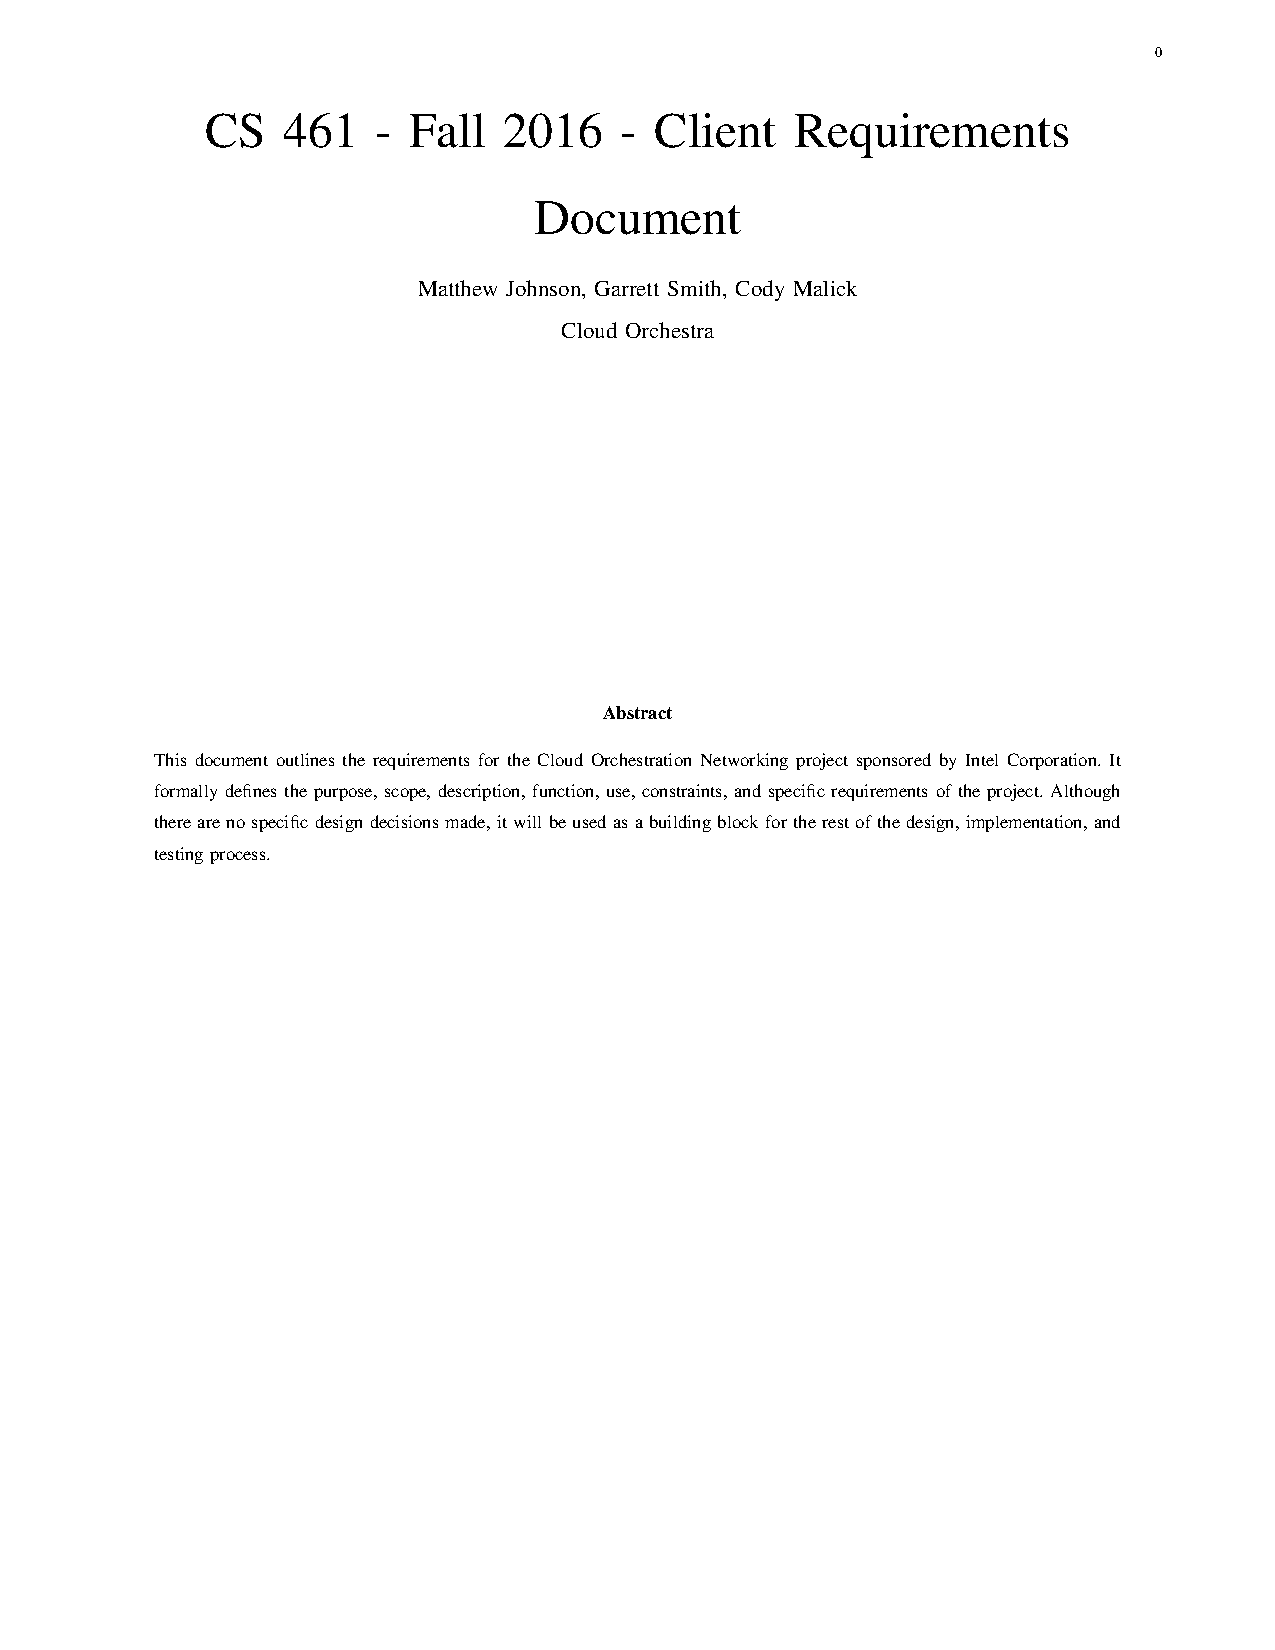
\includepdf[pages={-}]{docs/reqs.pdf}


\section{Project Evolution and Changes}
Our project goals over the year changed significantly. Large changing points were around
week seven of winter term, as we found that our implementation plan was not feasible. 

\subsection{Scope Change}
 Originally, we were planning on replacing the Linux tunnels with Open vSwitch generated
 tunnels. This ended up not being possible, as the Open vSwitch management database requires
 a full stack implementation. Specifically, we had to generate the the original endpoint,
 known as a bridge, and tunnels with Open vSwitch. As a side effect of having to restart the
 project week seven of winter term, we moved VxLan and NvGRE implementation to a stretch
 goal. This was approved by the customer.
 
\subsection{Table of Specific Changes}
Shown below are the itemized list of changes make to our project after the initial design
documents.

% Turning this into an official latex figure using \begin{table} displaces it in the document.
% Not worth the time to sort out now, would rather focus on finishing.

% \begin{table}[]
% \centering
% \caption{Table of changes}
%  
\begin{tabular}{|p{.5cm} |p{5cm}|p{5cm}|p{5cm}|}
\hline
\multicolumn{4}{|c|}{Scope Changes} \\
 \hline
\# & Original requirement & What happened to it & Comments \\ \hline
1 & Implement OVS Tunnels into Ciao & Found goal to be impossible without bridges and tunnels
    both originating from OVS & Occurred week 7 of winter term, approved by client  \\ \hline
2 & VxLan/nvGre Implementation & Became a stretch goal due to time constraints on the project
    & Should be a simple change once our changes are merged into Ciao \\ \hline
\end{tabular}
% \end{table}

\subsubsection{Final Gantt Chart}

%Uses package pgfgantt
\section{Gantt Chart}
Following is the actual distribution of work that occurred over the year. It is only slightly
different than our original projections, mainly in spring term. Due to the scope change, we
ended up working through the first four weeks of winter term to get the prototype in a working
state. The list item "original implementation" refers to work done before the scope change.
Lastly, we group bridge and tunnel implementation due to the fact that one does not work
without the other:\\

% Gantt chart location
\begin{ganttchart}[
		hgrid=true,
		vgrid={*{10}{blue, dashed}},
		y unit chart=0.75cm,
		x unit=1.5cm
	]{1}{9}
\gantttitle{2016-2017}{9} \\
\gantttitlelist{9,10,11,12,1,2,3,4,5}{1} \\
\ganttgroup{Project Documentation}{1}{4} \\
\ganttbar[progress=100]{Problem Statement}{1}{2} \\
\ganttbar[progress=100]{Requirements Document}{2}{3} \\
\ganttbar[progress=100]{Design Document}{3}{4}  \ganttnewline
\ganttgroup{Implementation}{4}{7} \ganttnewline
\ganttbar[progress=100,progress label text={}]{Original Implementation}{4}{6} \\
\ganttbar[progress=100,progress label text={}]{Open vSwitch Bridges and Tunnels}{6}{9} \\
\ganttgroup{Presentation}{7}{9} \\
\ganttbar[progress=100,progress label text={}]{Build Presentation Board}{8}{9}\\
\ganttbar[progress=100,progress label text={}]{Engineering Expo}{9}{9}
\end{ganttchart}


\section{Original Design Document}

\includepdf[pages={-}]{docs/design.pdf}

\subsection{Design Changes}
As stated in the scope change section, the primary changes were that we had to do a full stack
implementation. To summarize the change, we originally were required to do a re-implementation
of the linux-created GRE tunnels using Open vSwitch. After testing we discovered that Open vSwitch
does not recognize linux-created bridges due to the internally-managed state in the OVS database.
Therefore, all OVS-created GRE tunnels must attach to an OVS-created bridge. Originally, creating
OVS bridges and integrating them into Ciao was considered our stretch goal. With this revelation
we realized that creating the OVS bridges must be our first priority. This bumped the original
second goal to test NVGRE and VXLAN protocols into stretch goal status and the GRE tunnel creation
became our second goal. This approach required handling bridge creation and destruction as well
as creation of GRE tunnels and attaching them to the OVS bridge objects. This was essentially
integrating through the entire Ciao network stack.

\section{Original Tech Review}
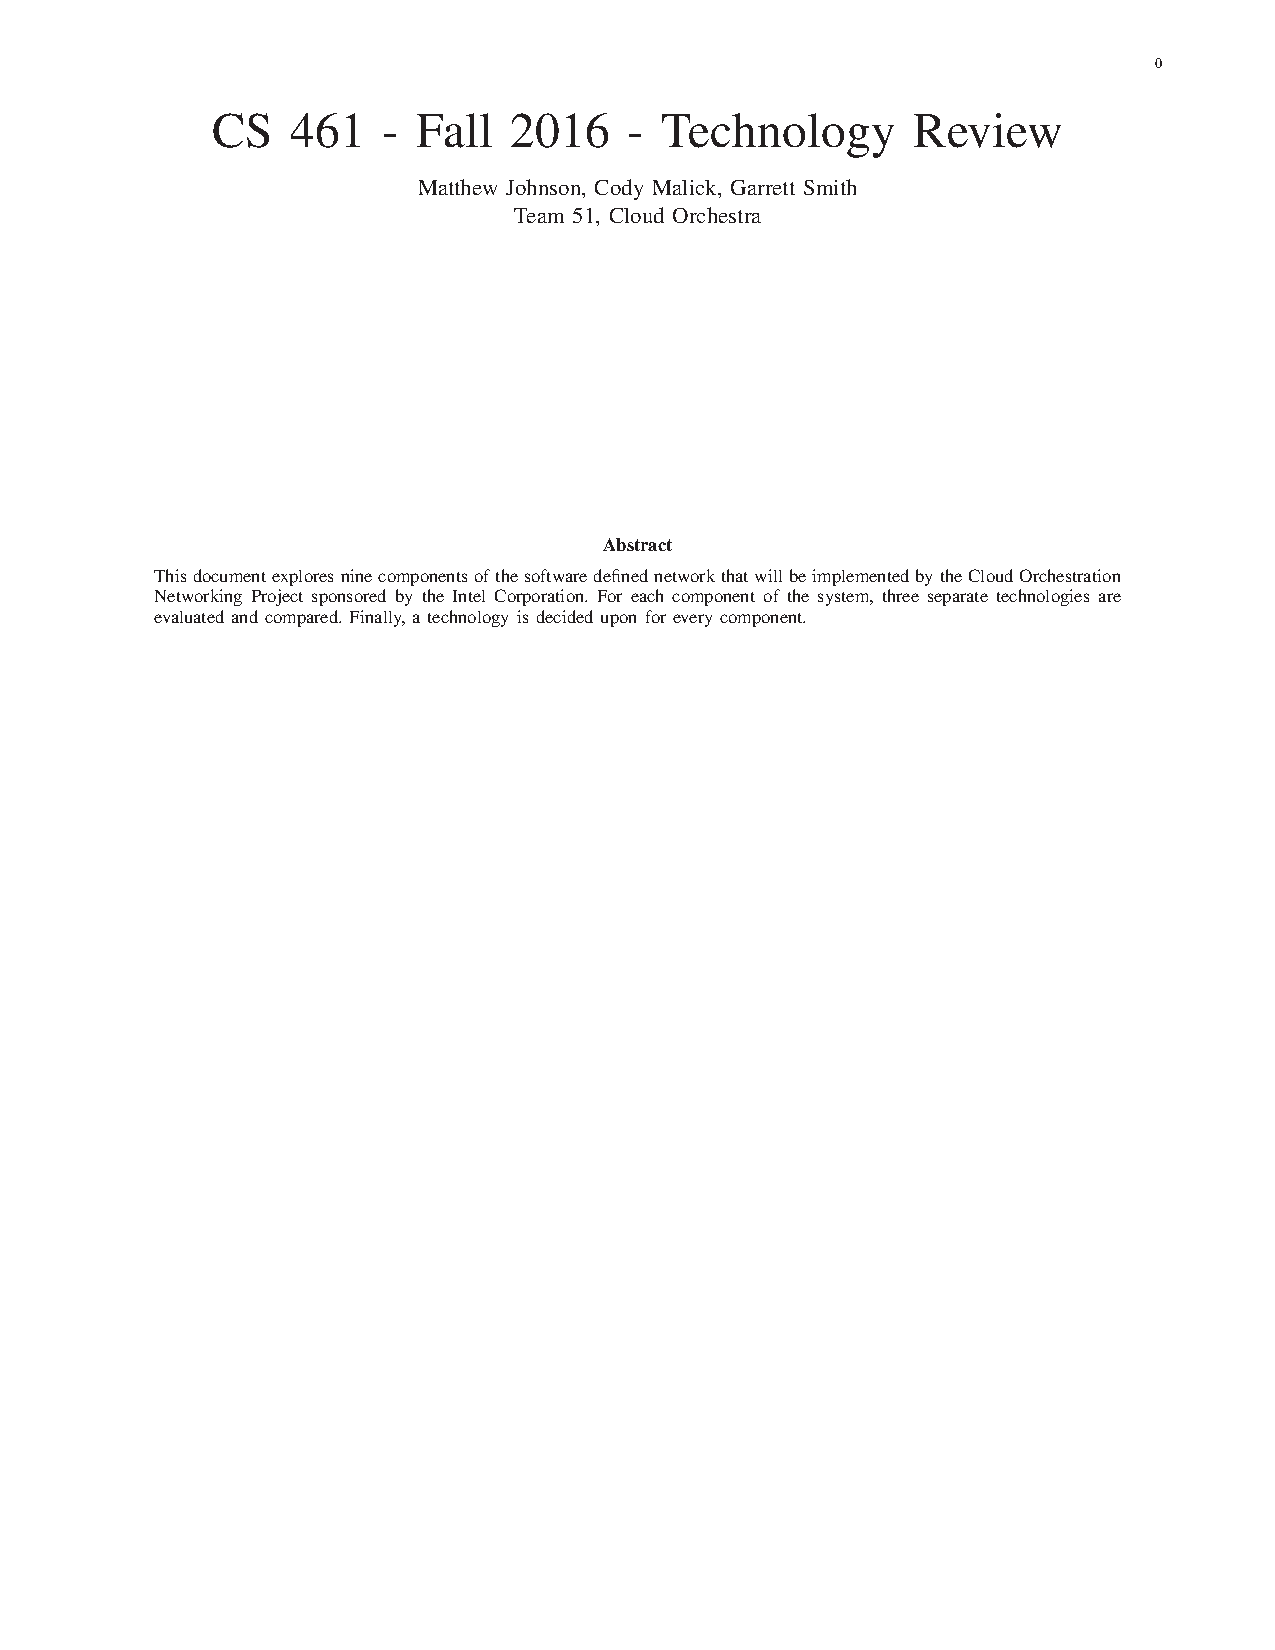
\includepdf[pages={-}]{docs/tech.pdf}

\subsection{Tech Changes}
Our tech stack changed in one area: we did not use \texttt{libovsdb}, the third party Golang
library for Open vSwitch. We discovered that it added unnecessary overhead, and we opted to go
for a direct interface with the OVS command line utility. After struggling with libovsdb integration
into Ciao for several weeks, we communicated our issues to our client. Our client advised us to
simplify our work and simply use the OVS utility. This simplified our work strategy considerably,
since we did not have to manage table mutations for every network change, and instead could allow
the utility to manage it internally.

\section{Blog Posts}
\subsection{Matthew}
\subsubsection{October 14, 2016}

This is the first update for our project, so it will cover more than a
week's worth of progress. First, a little background about our
relationship with our client and how this project came to be\ldots{}

\paragraph{Background} 

Over the Summer, 2016, I worked as a Software Engineering Intern for the
Advanced Systems Engineering (ASE) group within the Open Source
Technology Center (OTC) that is in turn within the Software Services
Group (SSG) at Intel. So I was a SEI in ASE in OTC in SSG at INTC. If
you've ever worked at Intel that sentence doesn't offend you\ldots{} or
maybe it does, I guess that depends on your experience at Intel.

I had the good fortune to work with some of the smartest people I've
ever met. In an effort to continue working with them and continue
challenging myself, I wrote a proposal requesting my group sponsor a
Senior Capstone Project. I was successful. Not only did they
enthusiastically embrace the idea, but provided enough quality hardware
to be successful and enough mentorship to get us off the ground.

\paragraph{Progress} 

We have made some progress since being put on this project. A couple
weeks ago we all traveled up to Hillsboro to meet with our clients,
which turns out to include a couple Principal Engineers (PEs) who are
miles more technical than us. During this meeting, one of the PEs was
kind enough to spend an hour of his time explaining the more technical
aspects of Ciao (I'm assuming I don't have to go into an explanation of
our project here) and what they wanted us to do. Also during this
meeting, we collaborated to write our problem statement due in this
class. The next week we set up the hardware required to run Ciao in a
cluster and began the process to register our hardware with the
university so we could be granted IP addresses.

\paragraph{Issues} 

Since then we have been trying to jump through various hoops to get
ethernet access on the hardware. This has been a continuing battle that
we expect to be resolved soon. We need internet to use git, remote
updates of Ciao and Clear Linux, and remote access to the cluster. We
need \emph{wired} internet because Clear Linux is a datacenter OS, and
therefore does not even package the common wifi setup tools, such as
\lstinline!iw!, \lstinline!wifi-menu!, \lstinline!wpa-supplicant!, etc.

\paragraph{Next Steps} 

The next step is to install the Clear Linux OS on the five Intel NUCs in
the cluster. Once that has been done we can set up Ciao and take initial
measurements as a baseline. This baseline will be recorded so we can
take further measurements once we implement our new networking mode
using OVS.

-- Matthew Johnson

\subsubsection{October 21, 2016} 

Not much progress was made this week, though not for lack of trying.

\paragraph{Progress} 

This week was almost entirely devoted to figuring out networking for our
hardware, 5 Intel NUCs. As mentioned previously, these NUCs will make up
the control node and compute nodes for the cluster we will be running
and testing Ciao on. After several days of debugging and a 22-email
chain with the IT director at OSU, we are still blocked.

Other than debugging the networking with the IT director, we have
successfully installed Clear Linux on all NUCs. This was done by
bringing them all home and installing Clear on my home network. Tonight
we will also receive feedback for our first draft of the Problem
Statement. Hopefully we will have the feedback addressed by tomorrow
morning (Friday, October 21st), since I will be driving up to Intel and
will be able to get any changes approved and signed.

\paragraph{Issues} 

As I mentioned above, the issue with the networking is a big one.
Hopefully we can get this figured out when the IT director returns on
Monday.

\paragraph{Next Steps} 

The next step is to get networking figured out. This is a necessary step
because we need to use the network to ssh into the NUCs, as well as
communicate with the internet for github access and Clear Linux updates.

-- Matthew Johnson

\subsubsection{October 28, 2016} 

\paragraph{Progress} 

This week we spent most of our time writing the rough draft for the
requirements document. We have turned it in and it is definitely a good
start. We will polish it over the next week to turn in next Friday.

Another big update for this week is that we have networking! I had
another email conversation with Todd Shechter, who was at a loss as to
why we could not access the network on our NUCs. He granted us access to
the HP switch we had successfully connected via in the past. On
Thursday, I went to move all our NUCs to the new switch. On a hunch I
decided to try out the network one last time. They all worked! Our
hardware is now set up and hopefully we will be able to get to work
soon.

\paragraph{Issues} 

No issues currently, except for an increased workload from other
classes. This being week 5, we all had midterms to contend with as well.
Hopefully things calm down for a couple weeks.

\paragraph{Next Steps} 

The next step is to finish our requirements document and get it signed
next week. We should also get Ciao installed on our NUCs and our cluster
set up.

-- Matthew Johnson

\subsubsection{November 4, 2016} 

\paragraph{Progress} 

This week we finished writing the requirements document that was due
today. After the rough draft we turned in last week we continued working
on it ourselves until Tuesday. On Wednesday Frank emailed us some
suggestions (thanks Frank) and we addressed those right away. We got the
document signed that afternoon by Rob Nesius, our client at Intel. We
will soon be receiving a book from Intel on SDN basics that will help us
get started with implementation. We would have liked to be starting on
implementation by now but the writing-intensive course load has tied up
our time a bit.

\paragraph{Issues} 

Our workloads continue to be heavy, but that won't change. We are doing
fine, completing our assignments on time, and have no immediate
blockers.

\paragraph{Next Steps} 

Our requirements document is turned in, so now we are looking ahead to
the design document. Hopefully we will also find time to start working
on setting up our cluster in the next couple weeks.

-- Matthew Johnson

\subsubsection{November 11, 2016} 

\paragraph{Progress} 

This week we started working on the technical review document due next
Monday. This document outlines nine different components of our system.
For each component we are exploring three different technologies that
could be used to implement the component. Since our project is
implementing a component of a larger system, it was difficult for us to
come up with nine components and three technologies each (twenty-seven
different options). We spent much of our week working together to figure
out how to split the project up. We will all be working on our portions
of the document over the weekend.

\paragraph{Issues} 

The biggest issue with the technical review document is that our system
is a single component of a larger system, and is therefore difficult to
split up into nine different parts.

\paragraph{Next Steps} 

The biggest looming deliverable is the technical review document due
Monday. When that is complete we need to start on the very big design
document due in a couple weeks.

-- Matthew Johnson

\subsubsection{November 18, 2016} 

\paragraph{Progress} 

Over the last weekend we completed our technology review document,
coming in at just over 16 pages total. Unlike several other groups we
managed to complete and turn in our technology review on time. We are
all satisfied with the result. Since then we have shifted to working on
the design document that is due December 4th. This will be the largest
document we produce this term and mostly marks the end of the
documentation phase. The one document due after the design document is a
term status report, which is mostly a combination of all the weekly
updates we have written to give a coherent picture of our progress so
far this year.

\paragraph{Issues} 

No issues currently.

\paragraph{Next Steps} 

The next big step is the large design document due at the beginning of
next month. We will be working on that over the next couple of weeks.

-- Matthew Johnson

\subsubsection{November 25, 2016} 

\paragraph{Progress} 

This was a short week with Thursday and Friday given over to the
Thanksgiving holiday. We have transitioned to using the template
requested by Kirsten for the design document and are ready to start with
writing the document and preparing for our final presentation.

\paragraph{Issues} 

No issues currently.

\paragraph{Next Steps} 

The design document is our most immediate concern, followed closely by
the end-of-term status report and presentation.

-- Matthew Johnson

\subsubsection{December 2, 2016} 

\paragraph{Progress} 

This week we focused on the design document due Friday. We spent time
researching design strategies and writing up our plan to execute. During
this research we found a very useful Go library that interfaces with
Open vSwitch. This library will simplify our implementation, allowing us
more time to do network performance testing, which the client is very
interested in.

\paragraph{Issues} 

No issues this week, we all worked hard and got the document done.

\paragraph{Next Steps} 

We are going to write the final report and do the final presentation
this weekend. During Winter break we hope to start on the
implementation.

-- Matthew Johnson

\subsubsection{January 13, 2017} 

\paragraph{Progress} 

Over Christmas break Cody and I did some pre-work on the NUCs setting up
our development environment and trying to get Ciao set up manually. We
ran into some tough issues and communicated with the Intel team. The
Intel team pointed us to a much more recently updated setup document
that included automated deployment.

This week Garrett set up his development environment and we began to go
through the automated deployment guide. After a show-stopper for much of
this week we were able to continue with the deployment steps. Once
deployed we will do our initial network measurements for baseline
performance.

\paragraph{Issues} 

We ran into a show-stopper when Docker certification was broken in the
latest version of Clear Linux (the target distribution). This was
quickly fixed by the Clear development team and pushed external. We then
had to remove the docker certification cache and everything worked fine
again.

\paragraph{Next Steps} 

Next steps are to finish the Ciao deployment then gather initial network
measurements. Once that is done we can implement our solution and test
again.

\subsubsection{January 20, 2017} 

\paragraph{Progress} 

The docker issue was fixed and we were able to begin the Ciao
deployment. We have been working through several issues, see below for
details.

While Cody and I have been working on deployment, Garrett has been
writing scripts to collect network performance data between nodes. He
has made significant progress in parsing bandwidth data into csv format
for graphical representation.

\paragraph{Issues} 

This week we continued to work on the Ciao deployment via automated
ansible playbooks. We encountered several issues from the start and have
worked through them one by one. Issues included errors in the ansible
playbooks regarding yaml parsing and fqdn configuration. This type of
issue was resolved by hardcoding the playbooks for our specific setup.
We are now seeing a certification error that we will be working on this
weekend.

\paragraph{Next Steps} 

Next steps are to finish the Ciao deployment and finish tooling for
latency measurements.

\subsubsection{January 27, 2017} 

\paragraph{Progress} 

This week we were successful in deploying Ciao and beginning
implementation of Open vSwitch components. Garrett has begun working out
network measurements for our initial benchmarks. Progress is being made.

\paragraph{Issues} 

The first half of the week was spent debugging our Ciao deploy with
members of the Ciao development team at Intel. After several email
conversations and debug steps, we were advised to switch our operating
system to Ubuntu because of various certification issues in Clear Linux.
This, along with running from within a ciao-deploy docker container,
fixed all of our issues. This has allowed us to move forward.

\paragraph{Next Steps} 

The immediate next step is to finish collecting network statistics and
implement Open vSwitch-created GRE tunnels in Ciao (in the
\lstinline!gre.go! file).

\subsubsection{February 3, 2017} 

\paragraph{Progress} 

We have continued tentative development on the OVS modules for Ciao.
Some of the necessary functions have been written, but it has been
difficult to test this over the physical cluster. Garrett, who has
worked on the OSU network in the past, thinks the network may not be
assigning IPs to the cluster. The OSU network DHCP servers will not
assign an IP unless the MAC address has been registered with the
university. To get around this we may have to do single-vm setup or find
a way to set up the cluster independent from the OSU network.

Ciao provides ciao-down, a tool that helps set up a single-vm
environment for testing. This will be helpful once we get it spun up.

\paragraph{Issues} 

We are still having issues gathering initial network metrics due to
inaccessible nodes on our physical cluster. Garrett is working through
this but the best way to address this may be single-vm for now.

\paragraph{Next Steps} 

Getting ciao-down running is a priority so we can actually test the
modules we are writing. We are also continuing to write the modules.

\subsubsection{February 9, 2017} 

\paragraph{Progress} 

We have a schedule we are following, and our current goal was to
complete the OVS module by today. Although we have a module written, we
are unable to get it to integrate properly with the rest of Ciao. The
testing environment we are using is ciao-down, the single-vm setup for
Ciao. I think we are misunderstanding some things in the calling
hierarchy. I plan to work on it this weekend and communicate our issues
to our client early next week. I'm attempting to set up a bridge with
OVS as well as the GRE tunnel - which may not be strictly necessary. I
thought it would make it easier.

\paragraph{Issues} 

As far as the physical cluster goes, we realized that the OSU network
will not lease IP addresses unless the MAC address is registered with
the University. Since Ciao uses the network's DHCP server to assign IP
addresses to the nodes this is a big issue. Garrett has been setting up
the physical cluster with a DHCP server running on the switch, with only
our deployment NUC connected to the internet. He has been running into
issues setting up the Keystone server once he took our controller NUC
off the internet. He was trying to modify ansible tasks to get around
the issue when I left campus today. If he isn't able to get this to work
we will probably ask the university for a subnet we can run a
non-MAC-locked DHCP server on, but Garrett has worked in OSU IT before
and said we are unlikely to get permission for that. The number of
errors the OSU network has generated for us has been a little
frustrating.

\paragraph{Next Steps} 

I'll continue working on integrating the module. If I have no luck I'll
work with the client next week to see what we are doing wrong.

\subsubsection{February 17, 2017} 

\paragraph{Progress} 

The majority of this week was spent preparing the Winter midterm report
and presentation due on Friday.

Early in the week I met with Manohar Castelino, the networking expert on
the Ciao project. Together we determined that OVS bridges are required
to interface with OVS tunnels and this significantly changes the scope
of our project. See our midterm report and updated requirements document
for more detail. This makes the stretch goal, OVS bridge implementation,
a primary goal along with creating the OVS tunnels.

\paragraph{Issues} 

No issues this week other than the scope change and associated goal
reorder.

\paragraph{Next Steps} 

Next week we will continue implementing an entire OVS framework for
Ciao, network bridges included.

\subsubsection{February 24, 2017} 

This week we made considerable progress in writing a framework for the
entire Open vSwitch network system. This was a new requirement
identified only last week, causing a scope change for our project.
Currently we have a framework written, but it is not integrated into
Ciao. That is our future work. Currently Garrett is working on testing a
DHCP server attached to an OVS bridge, which is required by the Ciao
CNCIs.

\paragraph{Issues} 

No major issues this week.

\paragraph{Next steps} 

Integrate the new framework into Ciao and complete DHCP-OVS bridge
testing.

\subsubsection{March 3, 2017} 

\paragraph{Progress} 

This week I moved houses, so my work was limited to the second half of
the week. I worked on polishing the OVS framework for Ciao. I found that
integrating into Ciao proper was extremely difficult because it is
necessary to practically rebuild Ciao networking from the ground up. I
spoke with Manohar Castelino about the scope of the project and he told
us he is okay if we just call out to the OVS commandline tool instead of
requiring direct API interaction. This has the potential to greatly
simplify our project and hopefully we can get back on track.

\paragraph{Issues} 

Personal issues this week with two of three team members inhibited
development. Those have been resolved and work continued in the latter
half of the week.

\paragraph{Next Step} 

Exec command line tools to set up OVS instead of integrating complicated
API calls into a complicated virtual network. I will meet personally
with Manohar this next week as well.

\subsubsection{March 10, 2017} 

\paragraph{Progress} 

We made a lot of progress this week. I spoke with Manohar about the
difficulties we were seeing integrating the OVS API into Ciao, and he
advised me to use the OVS command-line interface. Once this decision was
reached, we were able to quickly spin up some functions that
accomplished what we had been trying to accomplish with libovsdb all
along.

Once the functions were written I began integration work into Ciao
itself. Right now the integration is in place, but I have had trouble
seeing where the network mode is actually set in Ciao. This is my next
step.

\paragraph{Issues} 

No significant issues for me this week.

\paragraph{Next Steps} 

The next step is to demo our progress to our TA and finish integration
work into Ciao.

\subsubsection{March 17, 2017} 

\paragraph{Progress} 

This week we worked both on implementation and on creating a poster
draft for the expo. We submitted the poster before the due date and
switched our focus to implementation again.

I found an issue with our GRE tunnel creation code where we were not
configuring the port properly with the IP address. A simple call to
ifconfig configures the port.

Cody and Garrett found that we were not tracking bridge creation
correctly in Ciao, causing Ciao to think that bridges were not created.
They are working on this issue.

\paragraph{Issues} 

Ciao builds successfully, but it fails to actually connect the nodes.
This is our ongoing work.

\paragraph{Next Steps} 

Continue to debug why Ciao is not connecting the nodes.

\subsubsection{April 7, 2017} 

\paragraph{Progress} 

Over Spring Break I was lucky enough to attend a three-day Ultimate Go
programming language class provided by my work. Since this project is
being completed in the Go programming language it was highly relevant.

When we arrived back for Spring term we started working again. We
fleshed out some areas where Ciao needed to track our bridge creation
better. I discovered on Wednesday that Open vSwitch was not being
created on the compute nodes like we expected to.

\paragraph{Issues} 

The main issue causing failure was the failure to install OVS on the
compute nodes. I emailed Manohar and we received a response with how
that can be accomplished later in the week.

\paragraph{Next Steps} 

We really need to get this development finished as expo is fast
approaching.

\subsubsection{April 14, 2017} 

\paragraph{Progress} 

This week I identified a bug in our implementation that was creating
internal ports with the same name as the external-facing GRE ports. This
was causing the external port creation to fail and preventing workload
instances from being successfully created. When this was resolved (along
with a couple other minor issues), we were able to create instances
using OVS networking. While this represented a success and an important
step towards completion, we are still having issues. The instances are
ping-able (well, the compute node is, the instances are on separate
ports, and ports are not ping-able), but we are unable to ssh into them.
This is obviously a pretty big problem.

Cody and Garrett moved the NUCs to Cody's apartment to attempt physical
cluster setup without OSU network restrictions. Once the physical
cluster is set up we can gather network metrics on the hardware. We also
worked on the poster draft and had our group picture taken.

\paragraph{Issues} 

Right now the main issue is a failure to connect the OVS bridge to the
VNIC. The ovs-vswitchd logs indicate a netdev error, which I have been
unable to root cause. The specific error is as follows:

\begin{lstlisting}[language=bash]
2017-04-13T19:05:22.712Z|00016|netdev_linux|WARN|<bridge id>: obtaining netdev stats via vport failed (Invalid argument)
\end{lstlisting}

Then I see a lot of \lstinline!file not found! errors with the bridge
name as the file name.

\paragraph{Next Steps} 

Obviously, the next step is to figure out what the heck is going on with
OVS here. We will also complete the poster and submit it Monday.

\subsubsection{April 21, 2017} 

\paragraph{Progress} 

This week we rolled back some recent experimental changes to Ciao's VNIC
creation process in attempts to manage most of this via OVS. This was
unsuccessful and caused the previously ping-able instances to be
completely unavailable. We are now double checking that we are treating
CNCIs and CNs the same way. A discrepancy here could cause problems.

We also have worked on finishing our poster and have responded to
feedback from our client. Intel branding has been approved and the
finishing touches to the poster are being made.

\paragraph{Issues} 

No new issues this week.

\paragraph{Next Steps} 

Finalize the poster and continue to debug the network issues.

\subsubsection{April 28, 2017} 

\paragraph{Progress} 

We worked on the poster this week as well as cleaning up our log
statements for final code pull. The poster was approved by our client
after some revision requests, which were made. The poster was submitted
on Friday.

\paragraph{Issues} 

None

\paragraph{Next Steps} 

Wired review next week.

\subsubsection{May 5, 2017} 

\paragraph{Progress} 

This week we paired off with people from outside our group to conduct
the Wired-style review. We also emailed our code to Manohar so he can
look over what we have. We explained where we were stuck and asked him
to look over it and see if there were any glaring errors. When we
described our progress (that we can ping the instances but not ssh in)
he said it is probably just a very small configuration issue that is
preventing this from working fully.

\paragraph{Issues} 

None

\paragraph{Next Steps} 

Midterm report and video presentation coming up next week.

\subsubsection{May 12, 2017} 

\paragraph{Progress} 

This week we finished the Spring midterm video presentation and have
been working on the written progress report. We are still awaiting
feedback from Manohar on our code base if he has any.

\paragraph{Issues} 

No new issues this week. We thought we had broken the implementation
again when demoing for our video presentation, but it turned out to be a
simple configuration error.

\paragraph{Next steps} 

Turn in the progress report and prepare for expo next week.

\subsubsection{May 19, 2017} 

\paragraph{Progress} 

This week we submitted our midterm report/presentation on time. On
Friday we presented at the Engineering Expo. The expo went well.

\paragraph{Issues} 

Nope

\paragraph{Next Steps} 

Final writing assignments to be assigned Wednesday.

\subsubsection{May 26, 2017} 

\paragraph{If you were to redo the project from Fall term, what would
you tell
yourself?} 

I would probably remind myself to test early and test exhaustively. Much
of our early work was done in research, preparation, and setup. We found
out halfway through Winter term that the specific technologies we were
trying to integrate (Linux bridges and Open vSwitch GRE tunnels) were
incompatible with each other due to the database nature of Open vSwitch.
None of our research and proof-of-concepts with just Open vSwitch
indicated this. If we had taken time early to test how our project would
work with the exact combination of technologies we had to use, we could
have caught our scope change earlier, possible Fall term instead of
Winter term.

\paragraph{What's the biggest skill you've
learned?} 

At the beginning of this year I knew \emph{very} little about
networking, particularly software-defined networking. Because of this
project I have gained experience with Open vSwitch and cloud
orchestration technologies. I had to go from 0-60 in a relatively short
amount of time (well, maybe 0-55).

\paragraph{What skills do you see yourself using in the
future?} 

I think Go programming will be pretty valuable in the future. It is a
great new language that solves a lot of the security issues seen in C,
while still providing that low-level control that makes C so attractive.
I would like to do future projects using Go.

\paragraph{What did you like about the project, and what did you
not?} 

I loved when things worked, I did not love when they did not
work\ldots{}

Seriously though, it was great to trouble-shoot some of the issues we
were having and see positive results. Honestly, Open vSwitch is not
terribly complicated to use, but integration with Ciao was exceedingly
complicated. I think our remaining error has to do with Ciao integration
rather than Open vSwitch issues.

\paragraph{What did you learn from your
teammates?} 

I learned a ton about networking from Garrett. He came into this project
with a much better understanding of things than I did, and he was able
to correct many of my incorrect assumptions.

Cody has incredible organizational and people skills. He kept us on
track for due dates and insisted on high quality for our written
assignments. It is because of him our grades have been so high this
year. Cody also is very knowledgeable in Golang, and served as a great
human stack overflow when trying to remember go syntax.

\paragraph{If you were the client for this project, would you be
satisfied with the work
done?} 

I would be satisfied considering the scope change of the project. When
we had to implement both bridges and tunnels using Open vSwitch, it
changed how much of Ciao we needed to integrate with. The integration
was the hard part, not the actual bridge and tunnel creation.

\paragraph{If your project were to be continued next year, what do
you think needs to be working
on?} 

There is still the issue of not being able to SSH into the instances
that are created, so that needs to be addressed. Also, if feasible,
converting the go execs to actual libovsdb API calls would be nice, but
not necessary. I think the most important thing would be to complete our
stretch goal. Originally our second goal, network measurements using
NVGRE and VXLAN was moved to a stretch goal after our scope change.

\subsection{Garrett}
\subsubsection{October 14, 2016} 

\paragraph{Background} 

I'm interested in systems and infrastructure development and I would
like to focus on it after I graduate. When Matthew asked me if I wanted
to work on the Ciao project I was very excited. The project gives me the
chance to work on a piece of infrastructure software, learn about
software defined networking, and make a major contribution to an
important open source project.

\paragraph{Progress} 

A couple of weeks ago our team drove up to Intel's campus in Hillsboro
to meet with our clients.\\
They went over Ciao's network stack with us, explained the project in
depth, and answered questions. In addition to going over Ciao with us,
they helped us write an abstract and problem statement for the project.
We submitted the abstract and problem statement for the project on
Thursday afternoon (2016/10/13).

Intel is lending us 5 NUCs (small form factor computers), and a managed
Cisco switch to use as our datacenter for the project. Kevin McGrath is
giving us access to his lab so we have a secure place to set up the
hardware. We have the hardware physically in place in Kevin's lab, but
we need wired network access to install Clear Linux on the NUCs and set
up Ciao. We requested network access but the request has not yet been
approved.

\paragraph{Issues} 

We are still waiting on access to OSU's wired network for the 5 NUCs and
the switch that Intel are loaning us for the project. Network access is
required to install Clear Linux, Ciao, and access the machines remotely.
If we are unable to obtain network access for the hardware on OSU's
network we will need to find somewhere else to house it.

\paragraph{Next Steps} 

We would like to get the network issues sorted out as soon as possible
so we can finish setting up the NUCs and switch. Once we have network
access we will install Clear Linux, set up Ciao, examine how Ciao's
network stack currently works, and gather performance metrics. The
performance metrics we gather will be used to compare Ciao's current
network stack implementation against ours.

\subsubsection{October 21, 2016} 

This week consisted of a lot of emails and not much progress. \#\#\#
Progress \#\#\#\# Paperwork Our problem statement was reviewed and
returned to us without any feedback. Cody emailed Kevin asking if we
still need to resubmit the problem statement. We do.

\paragraph{Hardware and Software} 

In the land of NUCs and networks we are still having problems connecting
the NUCs to OSU's network. Todd set us up with two 5 port switches in
Kevin's lab, but we are having problems using them to connect to the
network. Clear Linux requires network access to install, but network
access requires us to set a hostname. We worked around the problem for
NUC number 1 by bridging my laptop's wireless connection to the NUC over
ethernet. This was a temporary workaround that let us install Clear
Linux and set a hostname for the NUC. Unfortunately once the NUC was
configured, we were still unable to obtain an IP address from the OSU
network using the switches Todd provided. Several emails with Todd later
we had NUC number 1 plugged into port 25 of the big 25 port switch in
the middle of the lab, and connected to the network. This means the NUCs
are configured correctly, and the issue likes somewhere in the network.
At this point Todd emailed us that he was out of the office until next
week, putting our network setup on pause. In the meantime, Matthew took
the other 4 NUCs home and installed Clear Linux on them there.

\paragraph{Issues} 

As I said above, we are having problems getting the NUCs connected to
OSU's network. Todd has been very helpful, but between email latency,
and school and work schedules consuming chunks of the day the networking
issues are taking a long time to resolve.

\paragraph{Next Steps} 

We need to work with Todd next week to get network access for the NUCs
in Kevin's lab. If that goes through we will set up Ciao on the NUCs.
Our problem statement does not require any edits so we will resubmit it.
The requirements document is due on the 28th so we will be working on
that.

--Garrett Smith

\subsubsection{October 28, 2016} 

\paragraph{Progress} 

The network issues have been solved. Matthew was going to move the NUCs
from the small Cisco switches Todd provided us to the large HP switch in
the middle of the room when Matthew discovered that the NUCs were able
to connect to the network using the small switches. Many thanks to Todd
Shechter for his assistance as we worked through the network issues. All
five NUCs have access to OSU's wired network. Now we can access them
remotely and configure Ciao.

In documentation land we submitted the rough draft of our requirements
document.

\paragraph{Issues} 

We didn't have any issues with the Capstone project its self. Between
midterms, homework for other classes, and attending the career fair I
was very busy which left less time to work on capstone.

\paragraph{Next Steps} 

The requirements document is due next Friday (2016/11/4) so we will be
working on it next week. We will also set up Ciao in its current form on
the NUCs.

-- Garrett Smith

\subsubsection{November 4, 2016} 

\paragraph{Progress} 

The final version of our requirements document has been signed and
submitted. I think we would like to be furhter along in setting up the
project and starting the implementation, but the writing requirements of
the class have kept us busy.

\paragraph{Issues} 

There haven't been any issues with the class or eachother. We are making
progress.

\paragraph{Next Steps} 

Next up is the design document. At some point we need to finish getting
the NUCs set up with Ciao, but right now the class is focusing on
documentation so we will be working on that primarily. Intel purchased
each of us a copy of a book on software defined networking that is
supposed to be arriving soon. I'm looking forward to digging into that
and learning more.

-- Garrett Smith

\subsubsection{November 11, 2016} 

\paragraph{Progress} 

This week we started work on the technology review. This involved
splitting our project into 9 parts and assigning 3 to each member of the
team. The goal of our project is to implement part of a larger system,
so finding 9 smaller parts was difficult. After meeting two separate
times we were able to figure out how to split the project into 9 parts.
Each of us has 3 parts to work on now, and we will be completing those
over the weekend.

\paragraph{Issues} 

There were no issues this week.

\paragraph{Next Steps} 

The technology review is due this coming Monday. We will be working on
it over the weekend. After the technology review is complete, we will
focus on the design document.

-- Garrett Smith

\subsubsection{November 18, 2016} 

\paragraph{Progress} 

This past Monday (2016/11/14) we submitted the tech review document. It
was a lot of work, but we got it in on time unlike many other capstone
groups. I researched software switch options, network latency tools, and
network throughput tools. For the software switch, Open vSwitch, the
software switch recommended by Intel, was the best option. Nothing else
I found came close in terms of features and portability. There were a
lot of options for tools that measure network throughput and latency. I
had a lot of choice when it came to choosing tools so I spent a lot of
time reading recommendations, looking at all of the options, and
comparing them to determine what would work best for us. Even though
using the tools isn't part of the assignment, I was curious about how
the networking tools I was researching worked so I set up and used some
of them to get more of an idea of what I would be doing.

\paragraph{Issues} 

We didn't have any issues this week.

\paragraph{Next Steps} 

The design document is out next big assignment. We will be working on it
over the next couple of weeks.

\subsubsection{November 25, 2016} 

This week was shorter due to the Thanksgiving holiday.

\paragraph{Progress} 

This week was short due to the Thanksgiving holiday. We met and
discussed how we will be completing the design document and progress
report. We have the design document laid out using the template Kirsten
wants us to use. We received feedback from Kirsten on the tech review.
Some of the feedback was helpful generally like watching out for spacing
issues.

In more of a personal progress report, I have been reading through the
book on Software Defined Networking. It is very insightful, and I wish I
had it at the start of the term.

\paragraph{Issues} 

No issues this week. The holiday is cutting into project time, but that
is unavoidable.

\paragraph{Next Steps} 

I will continue reading through the book on software defined networking.
The next big assignment that is due is the design document so we will be
working on it next week.

-- Garrett Smith

\subsubsection{December 2, 2016} 

\paragraph{Progress} 

This week we finished the design document. We each wrote up part of the
design, then spent time editing and revising the document. We turned in
the signed copy by the due date and did not need to turn in an unsigned
copy. It feels good to have the first iteration of the design document
complete because we are now in a position where we can work on
implementing the project over winter break.

\paragraph{Issues} 

No major issues this week.

\paragraph{Next Steps} 

The progress report is due Wednesday next week so we will be focusing on
that. We need to write both the presentation slides, and the document.
Our plan is to meet up on Sunday to record the voiceover for our
presentation.

-- Garrett Smith

\subsubsection{January 13, 2017} 

\paragraph{Progress} 

I got my dev accounts set up on the NUCs. We met up and worked on
getting Ciao set up.

\paragraph{Issues} 

We are unable to fetch remote docker images from docker.io because of a
certificate error. For example, trying to fetch the Cio setup image
results in the following error:

\begin{lstlisting}
garrett@fw-dear205-ciao-nuc0 ~ $ docker pull clearlinux/ciao-deploy
Using default tag: latest
Pulling repository docker.io/clearlinux/ciao-deploy
Error while pulling image: Get https://index.docker.io/v1/repositories/clearlinux/ciao-deploy/images: x509: certificate signed by unknown authority
\end{lstlisting}

At the time of writing this \lstinline!swupd! reports our software is up
to date.

\begin{lstlisting}
swupd-client software update 3.7.4
   Copyright (C) 2012-2016 Intel Corporation

Attempting to download version string to memory
Update started.
Version on server (12680) is not newer than system version (12680)
Update complete. System already up-to-date at version 12680
\end{lstlisting}

Ciao has a nice automated setup utility that is run using docker. With
docker down we can not use that. We were also planning on running the
network analysis tools for latency and bandwidth measurement in docker
containers. Docker not functioning is a blocker for us.

\paragraph{Next Steps} 

\begin{itemize}
\item
  Gather network performance metrics for latency and bandwidth between
  nodes on the SDN.
\item
  Implementation.
\end{itemize}

\subsubsection{January 20, 2017} 

\paragraph{Progress} 

Matthew and Cody have been setting up Ciao using the automated deploy
docker image. They have had a few issues with the set up, but they are
making progress.

I have been working on Ruby scripts to parse the output from iperf and
qperf into CSV format so it is easier to work with. iperf was pretty
simple to set up because it has an option to output its data in JSON
format which is easy to parse. qperf does not have a computer friendly
output option so the script for parsing its output is more complex. I am
familiar with Ruby and it has strong native support for string
manipulation so I chose it for this task.

\paragraph{Issues} 

We are having a cert issue with setting up Ciao that Cody and Matthew
are working on.

\paragraph{Next Steps} 

\begin{itemize}
\item
  Get the automated deploy working for Ciao.
\item
  Finish up the script that parses the qperf output into a CSV.
\end{itemize}

\subsubsection{January 27, 2017} 

\paragraph{Progress} 

Great success! Ciao is up and running on the 5 Nucs. Now we can go full
tilt on implementation.

\paragraph{Issues} 

We had some issues getting with the \lstinline!getfqdn()! call returning
the host name instead of the fully qualified domain name on Clear Linux,
and a few issues getting the security certs set up for Ciao on Clear
Linux. We switched to Ubuntu 16, after which we were able to get Ciao
running.

\paragraph{Next Steps} 

I will be gathering network performance statistics over the next few
days while we figure out how to set up OVS GRE tunnels.

\subsubsection{February 3, 2017} 

\paragraph{Progress} 

We worked on the development of an OVS module for Ciao so we can get OVS
GRE tunnels implemented. Cody and Matthew have been spearheading that
while I have been troubleshooting issues with the multi machine
deployment of Ciao. More on those below. As a workaround, and to help
with development we are going to set up Ciao-down which is a single
machine deployment of Ciao.

\paragraph{Issues} 

Our deployment of Ciao on the 4 NUCs is not functioning correctly. We
are unable to deploy new workloads which is preventing me from running
gathering network performance statistics. When trying to run a workload
the Ciao controller generates a 500 error:
\lstinline!{"error":{"code":500,"name":"Internal Server Error","message":"Unable to Launch Tenant CNCI"}}!.
I dug into the source code and determined that this error message only
occurs when
\href{https://github.com/01org/ciao/blob/6eb98ce70d8b923bcdcedf628d68dd36645f9b87/ciao-controller/command.go\#L125}{the
CNCI does not have an IP address}.

I was lurking in the Ciao IRC channel when there was a discussion about
moving CNCIs. One of the details of moving a CNCI is is that it has its
IP address assigned by the underlying physical network. OSU's network
will only assign IP addresses to machines with registered MAC address.
This a a problem if we are going to be spinning up VMs on the fly. I
have not confirmed this is the issue but it looks like a likely
candidate. I emailed the Ciao developers and Tim Pepper gave me some
tips for setting up more verbose error logging. I will be setting up
more verbose logging and errors to try to determine if the CNCIs are not
being assigned IPs, and to try to track down the root of the issue if
that is not the problem.

\paragraph{Next Steps} 

We are going to get ciao-down running so we can run and test ciao on one
machine. I will keep troubleshooting the multi machine deployment of
ciao so we can gather performance metrics.

\subsubsection{February 9, 2017} 

\paragraph{Progress} 

Matthew and Cody have been working on implementing OVS created GRE
tunnels. They have Ciao down running and have been developing using
that.

I moved our Ciao cluster off of the OSU network onto a LAN running off
of the switch Intel is lending us. I'm running the switch in layer 3
mode which allows me to use its built in DHCP server. I'm hoping this
will resolve the problems getting IP addresses for the CNCI VMs. I have
Nucs 0 through 3 connected to the LAN, and I'm working on getting Ciao
running on them. Cody is currently using Nuc4 for his development
environment.

\paragraph{Issues} 

I had some trouble getting the switch set up due to my unfamiliarity
with its configuration software which took one development day to get
working.

The current issue I am having is cleaning out the old configuration we
had set for Ciao. The Ansible deployment is still using the old hostname
(fw-dear205-ciao-nuc1.engr.oregonstate.edu) for Nuc1 when trying to
connect to the Keystone server which is breaking the deployment. Git
grep isn't showing the hostname as being hard coded anywhere in the
config, but it is coming from somewhere.

\paragraph{Next Steps} 

Next week I will figure out the configuration issues and start gathering
metrics. I also need to get an instance of Ciao down running so I can
help out with development.

\subsubsection{February 17, 2017} 

\paragraph{Progress} 

This week we spent most of our time working on the midterm progress
report.

Matthew met with Manohar Castelino, the Intel Ciao networking expert to
discuss a possible change in the scope of our project. We need to
implement our stretch goal of OVS bridges alongside of OVS tunnels
because OVS tunnels require OVS bridges.

\paragraph{Issues} 

Nothing major this week.

\paragraph{Next Steps} 

Next week its back to development. I will also spend some time working
on the network performance measurements.

\subsubsection{February 24, 2017} 

\paragraph{Progress} 

We made good headway on the OVS bridge implementation. I figured out
part of the configuration with the Ciao cluster.

\paragraph{Issues} 

Nothing major this week.

\paragraph{Next Steps} 

Continuing implementation and testing.

\subsubsection{March 3, 2017} 

\paragraph{Progress} 

This week I got docker containers connected to an OVS bridge.

\paragraph{Issues} 

Nothing major.

\paragraph{Next Steps} 

Get a DHCP server connected to the bridge and see if I can have it
assign IP addresses to the docker containers.

\subsubsection{March 10, 2017} 

\paragraph{Progress} 

This week we made some good progress. Right now we are calling the OVS
CLI tool in Go to create bridges. See Cody's blog post for more details
on how this works. This is easier to use, and faster on development time
than using a library. It should also simplify the process of creating
nvGRE and VxLAN bridges.

We discussed this with the client and they are fine with this approach.

I connected three docker containers to an OVS bridge, ran a DHCP server
in 1 of them, and had the other docker containers request IP addresses
from the DHCP server to confirm that the DHCP server in the CNCIs should
work with the OVS bridges.

\paragraph{Issues} 

I spent a little bit of time fighting with Docker and dynamically
assigned IP addresses. It ends up that

\paragraph{Next Steps} 

We need to add configuration to Ciao to enable switching between OVS and
Linux bridges.

\subsubsection{March 17, 2017} 

\paragraph{Progress} 

This week we worked on the poster. We submitted our first draft with
most of the information but no picture. Matthew has started commuting
from Portland, so getting everyone together for a picture was not
convenient this week. We will add one before the final poster submission
is due.

We made more progress integrating the OVS bridges into Ciao. Cody and I
looked into how the Bridge struct is used to create track bridges in
Ciao and we are modifying it to have the option for OVS bridges.

\begin{lstlisting}
func NewBridge(id string, mode NetworkMode) (*Bridge, error) {
    bridge := &Bridge{}
    bridge.Link = &netlink.Bridge{}
    bridge.GlobalID = id //TODO: Add other parameters
    bridge.Mode = mode
    return bridge, nil
}
\end{lstlisting}

\paragraph{Issues} 

We weren't all able to meet to get a picture for the poster.

\paragraph{Next Steps} 

Finals are next week so we will be working on the progress reports.

\subsubsection{April 7, 2017} 

\paragraph{Progress} 

Over break Cody and I spent some time pair programming and made
modifications to the Bridge struct that is passed around in Ciao. This
struct is used to track bridges, and we had been bypassing it when they
are created. We added a mode the the bridge to track OVS or Linux bridge
type, and modified the \lstinline!create()!, \lstinline!destroy()!,
\lstinline!enable()!, and \lstinline!disable()! methods to have
different behavior depending on which mode is set.

\paragraph{Issues} 

We spent about 5 hours on Wednesday working together in a collaboration
room and discovered problems with our dependencies. OVS is not being
installed on tenant VMs. We emailed Manohar and received instructions
for how the dependencies for tenants are configured so we are working on
modifying those to get OVS installed correctly as a dependency.

\paragraph{Next Steps} 

Development, development and troubleshooting. We need to get our
prototype working soon with expo fast approaching.

-- Garrett

\subsubsection{April 14, 2017} 

\paragraph{Progress} 

We made some changes to the vnic (virtual nic) part of the Ciao
networking library to allow us to attach the virtual interfaces to OVS
bridges.

We switched to single VM for development, but we still need to get Ciao
running on a cluster of machines. We moved the Nucs Intel is lending us
for the project out of the lab at OSU and into Cody's apartment and onto
his network. We have a lot more control over his network so hopefully we
will have a smoother deployment experience there.

\paragraph{Issues} 

We are getting errors when we try to attach the virtual network
interfaces to OVS bridges.

\paragraph{Next Steps} 

Get Ciao set up on the physical cluster running on Cody's home network.

\subsubsection{April 21, 2017} 

\paragraph{Progress} 

This week we continued looking into the issues with SSHing into the VMs.

We met with our client and Kirsten to discuss our progress and
expectations for expo. Finally, we worked on the poster for expo.

\paragraph{Issues} 

No new issues, but we are still having issues SSHing into the VMs.

\paragraph{Next Steps} 

Finalize what we have an prepare for expo. Finish up the poster.

\subsubsection{April 28, 2017} 

\paragraph{Progress} 

This week we got the poster finalized and submitted.

\paragraph{Issues} 

Nothing major this week.

\paragraph{Next steps} 

Final code cleanup in preparation for the code freeze.

\subsubsection{May 5, 2017} 

\paragraph{Progress} 

This week we had the Wired style review to work on. That took a few
hours, but I found it helpful because it gave me practice explaining our
very technical project.

On Sunday we submitted our expo poster.

We did some code cleanup, and emailed Manohar with our progress.

\paragraph{Issues} 

Nothing new this week.

\paragraph{Next Steps} 

Next week we need to work on the midterm report and video.

\subsubsection{May 12, 2017} 

\paragraph{Progress} 

We did the midterm progress report and video this week.

\paragraph{Issues} 

Nothing this week.

\paragraph{Next Steps} 

Expo is next week so we will be doing that.

\subsubsection{May 19, 2017} 

\paragraph{Progress} 

This week was expo. I went to expo and presented.

\paragraph{Issues} 

My feet hurt.

\paragraph{Next Steps} 

Do whatever is left in the class.

\subsubsection{May 26, 2017} 

\paragraph{Post Expo Summary.} 

This is the last blog post after expo.

\paragraph{If you were to redo the project from Fall term, what would
you tell
yourself?} 

We had a big scope change because it was assumed that we could use Open
vSwitch for just the tunnel endpoints. I would warn past me that this is
an issue. To generalize the advice I would say to spend more time
initially on proofs of concept and make sure that what we think we can
do lines up with what we can do. We spent a lot of time researching and
planning, but it would have been helpful to jump in with tools earlier
and learn how they work and interact.

\paragraph{What's the biggest skill you've
learned?} 

I learned a lot about networking, and specifically how software defined
networks work. I know I will need networking knowledge for the job I
have lined up after college, and working on this project gave me really
good practical experience with software defined networks.

\paragraph{What skills do you see yourself using in the
future?} 

Networking, networking, and more networking! I won't be focusing on
networking, but as I said before I will need networking knowledge at my
future job.

This was the first large project I have worked on in Go. I like the
language and I plan on using it again for personal projects.

\paragraph{What did you like about the project, and what did you
not?} 

Liked

Working on big software projects is always interesting to me, and I'm
glad we were working on a real world project with real applications. Go
is a great language. Before working on Ciao I had only touched it
briefly for a small personal project, working on a large Go project
taught me a lot about how it works. I have been interested in continuous
integration and cloud management for a couple of years now so working on
Ciao was great chance to get hands on development experience with cloud
software. Who you are working with can definitely make or break the
project. Matthew and Cody were great to work with, and I would
definitely team up with them again for other projects.

I wish we had known about the single machine dev environment from the
start. It would have made getting going easier, and relieved some of the
headaches we had with initial setup. There wasn't anything big I
disliked about the project.

\paragraph{What did you learn from your
teammates?} 

Matthew was provided great leadership. I learned how to deal with scope
change, and stay motivated when the project goes sideways like ours did
with the scope change.

Cody has the most Go knowledge. We sat down together and did some pair
programming which was very valuable. I would have spent a lot more time
on some of the code I wrote without his help. He also has ruthless time
management skills. He did an amazing job of keeping track of all of the
due dates, and making sure we were on track.

\paragraph{If you were the client for this project, would you be
satisfied with the work
done?} 
Yes, we had some big scope changes, but those were communicated with
our client. Getting Open vSwitch integrated into Ciao was the biggest
part of the project and we were largely successful at that.

\paragraph{If your project were to be continued next year, what do
you think needs to be working
on?} 

We aimed for proof of concept and functionality first which means that
there are a few places our code could be cleaned up. Some of the code we
wrote is for lack of a better term, hacky. We are interacting with Open
vSwitch using exec and the the OVS cli tools. That could be cleaned up
and refactored.

We didn't hit all of our stretch goals. If someone else were to pick
this up they should work on testing different tunneling protocols, and
trying to get DPDK working.

\paragraph{Closing Thoughts} 

I learned a ton on this project. It was very challenging at times, but
I'm glad I chose it because it was a unique learning experience. Matthew
and Cody were great group mates, and I want to thank them for inviting
me to work on the project with them. I also want to thank Rob Nesius and
Manohar Castelino, and Intel for sponsoring the project. They were great
work work with.

FIN,\\
Garrett

\subsection{Cody}
\subsubsection{October 14, 2016} 

This is my first blog post of this exciting senior project. For detailed
background information, see Matthew's update. He's done an excellent job
writing up how the project came to be.

\paragraph{Background}

I was approached by Matthew and invited onto the project. It is of great
interest to me for a number of reasons: + I am, objectively, a complete
greenhorn when it comes to infrastructure systems development. I often
find the best way to learn is by finding a project, and grinding my nose
against it for a time to learn. + There are few opportunities to work on
something as bleeding edge as Ciao. There are even fewer opportunities
to get work experience in developing software defined networks. Both of
these opportunities appealed to me greatly. + I wanted to learn golang
on my own time, and after finding out Ciao was in go, I could hardly
refuse.

After accepting, Matthew, Garrett, and I all went up to Intel during the
first week of classes and met the team. After a wonderful explanation of
the project, and what was expected of us, we set off to start getting
the project together.

\paragraph{Progress} 

We've set up the five NUCs, small Intel computers, that will act as our
``cloud.'' Once the project is all setup, we will be simulating a
production environment that we can test and deploy our project on. I
would like to thank Intel for providing such a wonderful and high
performance testing environment.

While visiting Intel, we also got our problem statement and abstract put
together and approved by the customer. The team has been incredibly
helpful, and efficient at getting us any information we need to get
moving on the project.

\paragraph{Issues} 

The only wall that we've hit is getting the networking capability set up
on campus. Because of the set up on campus, Network Services prevents
deployment of random Ethernet devices. A pragmatic policy to be sure.
Knowing all the mischief that college students get up to, I completely
understand why this policy is in place. Because of this, we need to get
approval from Network Services before our initial deployment of the Ciao
infrastructure.

\paragraph{Next Steps} 

Once the network issues are out of the way, we can move forward with our
initial testing setup with Ciao. Once that's set up, we can define what
the requirements of the project are, and begin designing what exactly
needs to be implemented.

Thanks for taking the time to read this, and look for future updates!

Ciao,

-- Cody Malick

\subsubsection{October 21, 2016} 

This week was a little less action packed than the last. Here's what's
happening this week:

\paragraph{Progress} 

We had our problem statement reviewed, and we're waiting on the feedback
from Kevin. That should arrive later tonight. We also spent some time
getting the five Intel NUCs (Next Unit of Computing) set up in the lab.
Matthew spent a good amount of time Wednesday getting them imaged with
Clear Linux, Intel's flavor of Linux. We also got the base latex files
for the requirements document pushed to a new branch of the docs repo,
``client\_req.'' We'll be updating that and merge it once the first
version is complete.

We also looked through the basic requirements of the requirements
document from IEEE.

\paragraph{Issues} 

Our issues with networking continue through this week. Todd, from the
engineering network team, has been incredibly helpful and prompt in his
responses. We plan on getting this issue resolved early next week.

\paragraph{Next Steps} 

After the network issues are ironed out, we'll get our test environment
set up with Ciao, and get our requirements document written up.

Until next week,

-- Cody Malick

\subsubsection{October 28, 2016} 

This week we wrapped up fixing the networking and submitted our
requirements document.

\paragraph{Progress} 

This week we submitted our finalized and signed copy of the problem
statement. With that out of the way, we switched gears into the
requirements document. We've worked through a rough draft, and will be
fleshing out the details over the weekend. The requirements document has
been good to read through, even in it's current form. It's given me a
little more insight into what exactly the project is, and how we're
going to go about design and implementation. Overall, I'm glad we're
doing one.

This week we also got our networking issues resolved! This is great news
as it will now allow us to completely configure and update our NUCs as
needed without having to be in the lab.

We met with Frank on Tuesday and gave him the update on where we're at
currently.

\paragraph{Issues} 

No notable issues this week. We're moving forward at a good clip.

\paragraph{Next Steps} 

We'll be completing the requirements document this coming week, as well
as working on configuring the current implementation of Ciao on our five
NUCs. We're also expecting some books from Intel that should give us
more insight and information into software defined networks.

Until next week,

-- Cody Malick

\subsubsection{November 4, 2016} 

This week we got our requirements document reviewed and signed by our
customer.

\paragraph{Progress} 

This week we submitted our finalized and signed copy of the requirements
document. It's been a rather busy week, but our team has been working
well together! We laid out a tentative plan for our next steps, which
involve the design document and getting the books we need to being
working with Software Defined Networks.

We met with Frank on Tuesday and gave him the update on where we're at
currently.

\paragraph{Issues} 

No notable issues this week. We're moving forward at a good clip.

\paragraph{Next Steps} 

The next major steps are the tech review documents due next week, and
begin work on the design document. We're supposed to be receiving a book
from Intel soon as well which should help us get started.

Until next week,

-- Cody Malick

\subsubsection{November 11, 2016} 

This was a fairly tame week. Here's the update:

\paragraph{Progress} 

We've moved forward on our Tech Review paper. We have the outline
detailed, and which person is working on each component. It was a little
difficult for us to break up the project into the individual components.
The main reason for the difficulty was that we are implementing a small
subcomponent of a very specific system. We ended up figuring it out, and
we'll all be writing our pieces this weekend.

\paragraph{Issues} 

No notable issues this week.

\paragraph{Next Steps} 

I will be working on the tech review this weekend, and we will have it
turned in on Monday.

-- Cody Malick

\subsubsection{November 18, 2016} 

\paragraph{Progress} 

It was a busy week! The team managed to get the Tech Review done on
time. It ended up being quite a bit of work for each of the components
the team was working on. My favorite section of the tech review was
covering the network protocols section. I ended up choosing SSNTP,
Simple Secure Network Transfer Protocol. The protocol was quite
interesting as it was custom tailored to our project's needs. It was
created by one of the principal engineers at Intel, who was also the
creator of the project. It builds off of the security and handshake
protocols that SSL and TLS established, but reduces the protocol
overhead by only needing to do the initial handshake once. There were
other sections, but they weren't nearly as interesting.

\paragraph{Issues} 

No issues this week, we're moving along very nicely.

\paragraph{Next Steps} 

We've started on the design document for the end of term. We'll be
adding to that incrementally in the coming weeks.

-- Cody Malick

\subsubsection{November 25, 2016} 

\paragraph{Progress} 

We had a short week this week. We've started on the design document. We
will be making the transition over to the template provided by Kirsten
for this assignment. In the last few documents, we had not used the
exact template she provided. We will be doing so for the final documents
this term.

Our team also got together and talked about how we were going to execute
the final presentation video for a few minutes this week.

\paragraph{Issues} 

No issues this week. One thing I could use more of, however, is time!

\paragraph{Next Steps} 

With the template setup on the design document, we're ready to move
forward with the bulk of the writing.

-- Cody Malick

\subsubsection{December 2, 2016} 

\paragraph{Progress} 

This week we wrote the design document up, and got it signed just in
time for submission on Friday. Writing the design document was helpful,
as it forced the team to read through what libaries and interfaces in
those libraries we need to use. As well as getting a somewhat formal
design plan in place, it gave us a more informed overview of what peices
of the project need to get done.

\paragraph{Issues} 

No issues this week! Everything is moving smoothly.

\paragraph{Next Steps} 

This weekend, the team is going to write the final report, and record
the final presentation. After finals, we're planning on getting into the
implementation bit of Senior Design before school starts.

See you in Winter Term!

-- Cody Malick

\subsubsection{January 13, 2017} 

\paragraph{Progress} 

Over break, Matthew and I got our developer accounts set up on each NUC,
and Garrett got his set up this week. We were only able to meet once
this week due to the weather, but we laid out a couple things to do to
get moving in development. I plan on building a more concrete list of
action items that we can complete next week.

\paragraph{Issues} 

We had a show-stopping problem trying to get Ciao set up this week. The
specific error and issues are detailed in Garrett's blog post. The issue
has since been resolved, and we're moving on to finish the deployment of
Ciao.

\paragraph{Next Steps} 

\begin{itemize}
\item
  Finish Ciao deployment
\item
  Create list of actions to move development forward
\item
  Start development
\end{itemize}

\subsubsection{January 20, 2017} 

\paragraph{Progress} 

This week was rough for the team, in that we have encountered quite a
few issues deploying Ciao. Matthew and I have spent most of our time
this week working through configuration changes in Ciao, and while
progress has been made, we have not yet successfully completed
deployment.

Luckily, Garrett has been making great progress by writing some scripts
that analyze network traffic statistics. Some progress has been made!
Wohoo!

If we can't get this sorted beginning with next week, we will reach out
to Intel and see what help they can provide.

\paragraph{Issues} 

As stated above, we encountered quite a few issues deploying Ciao.
Specifically, when Ansible is running, we've run into about five or six
major errors that halt production. While many of these have been
bypassed through modification of configuration files, we have yet to
have success in deployment.

\paragraph{Next Steps} 

We will continue to debug deployment, and start development on Ciao once
we have a working test environment.

\subsubsection{January 27, 2017} 

\paragraph{Progress} 

A small amount of progress was made this week, but in a big way. We
resolved our issues with ciao deployment! We were able to deploy ciao,
and start initial development and network testing. We want to pull
network statistics before we make changes, so that we can see what
improvements are made by our implementation.

\paragraph{Issues} 

Continuing from last week, we were having quite a few issues deploying
ciao. What we ended up finding out was that we were supposed to be
running our ansible commands from inside of a docker container. Once
that issue was resolved, deployment went relatively smoothly, thanks to
Garrett and Matthew's hard work.

\paragraph{Next Steps} 

Next steps are implementing Open vSwitch, and generating GRE tunnels
from OVS. We are excited to start development.

\subsubsection{February 3, 2017} 

\paragraph{Progress} 

This week, we started development on implementing the OVS interface into
ciao. We're working on understanding libovsdb, the golang library we've
chosen to ease development. We've written a couple functions, but have
found a need to set up ciao-down, a single environment, development
distribution that makes compilation and testing of ciao fast and easy.

I'm going to be working on setting that up over the weekend.

\paragraph{Issues} 

We are still having issues gathering initial network metrics. More on
this from Garrett's blog post.

\paragraph{Next Steps} 

I'm working on setting up ciao-down on a development machine, and will
be working on implementing OVS GRE tunnels over the weekend. We're
aiming to have a basic prototype of this feature working by the end of
next week.

Until then,

ciao

\subsubsection{February 9, 2017} 

\paragraph{Progress} 

This week we made progress into the first feature, implementing OVS
generated GRE tunnels. Matthew and I pair programmed a couple times this
week, but he made quite a bit of progress writing the code for bridge
creation.

Outside of working with Matthew, I got a development environment set up
for myself on NUC4, and can work on that remotely whenever I need. This
is great news, because I hit a lot of road blocks on my personal
machines trying to get this set up. I even went so far as to install
linux on my laptop, but I was not able to get nested KVM enabled.

Garrett also got a working network test environment working. We should
have initial network metrics soon.

\paragraph{Issues} 

I'm happy to say that our issues now are development related, not
logistics. The current issue is that we need to find all the places that
a bridge creation function call need to be filled in. I created a page
to attempt to map out all those locations
\href{https://github.com/codymalick/CapstoneDocs/wiki/GRE-Function-Call-Hierarchy}{here}

\paragraph{Next Steps} 

This coming week, we are getting our midterm progress report written,
and our goal is to get OVS GRE bridges working.

See you next week.

\subsubsection{February 17, 2017} 

\paragraph{Progress} 

This week was focused primarily on writing the midterm progress report.
Matthew met with Manohar, the main networking Engineer at Intel who
designed Ciao.

\paragraph{Issues} 

No issues this week.

\paragraph{Next Steps} 

Next week we will continue work on implementing OVS into Ciao.

Ciao,

Cody

\subsubsection{February 24, 2017} 

\paragraph{Progress} 

We made some good headway into the bridges this week. I managed to
figure out how to run a test on a single file, allowing us to see
compilation errors. Before, we were just running the local VM to see if
the code works. This is great, and allows us to see what state the code
is in before deploying it into Ciao-Down.

We also got our new documents signed and dropped them off as requested.

\paragraph{Issues} 

No issues this week. We're continuing development.

\paragraph{Next Steps} 

Next week we are aiming to ship a working prototype of the OVS bridge.

Cody

\subsubsection{March 3, 2017} 

\paragraph{Progress} 

Unfortunately I was out sick most of the week. Personally, I did not
make much progress. On Friday, Matthew and I briefly discussed the OVS
management DB, and he's going to fire some questions off to the folks at
Intel.

\paragraph{Issues} 

The big issue we've run into is that, from what we can tell, to get OVS
working we have to completely overhaul the networking component of Ciao.
This is quite the undertaking.

\paragraph{Next Steps} 

Once the questions are answered, we'll know more about what the next
steps are.

Cody

\subsubsection{March 10, 2017} 

\paragraph{Progress} 

This was a very good week for progress. After some discussion with the
client, we found that it was acceptable to use the CLI (command line
interface) for Open vSwitch directly. In contrast to using a third party
library, this is straightforward and trivial to call from Go. With this
new approach, we were able to replicate quite a bit of the work that had
been done thus far in libovsdb with direct command line calls.

Calling the CLI via go is easy. Here's an example of how we call the OVS
command line interface:

\begin{lstlisting}
func vsctlCmd(args []string) error {
    if _, err := exec.Command("ovs-vsctl", args...).Output(); err != nil {
        return err
    }

    return nil
}

func createOvsBridge(bridgeId string) error {
    // Example: ovs-vsctl add-br ovs-br1
    args := []string{"add-br", bridgeId}

    // Execute command
    if err := vsctlCmd(args); err != nil {
        return err
    }

    return nil
}
\end{lstlisting}

While it would be ideal to use an API, this method works well without
providing unneccesary overhead to the project. We're implementing all
the needed commands in Ciao, and are optomistic about getting a
prototype working before end of term. Another advantage of this approach
is that getting nvGRE and VxLan working are trivial. All it requires is
setting a string in the command arguments.

\paragraph{Issues} 

I've had an issue with my development environment this week.
Specifically that when I try to test the code new code, it isn't being
properly copied to the test VM via ciao-down. I haven't run into this
before, but I presume I'm doing something silly. I'll post an update on
this once I have it fixed.

\paragraph{Next Steps} 

Moving into dead week, I'm confident of our ability to get a Ciao
prototype working. I will be focusing on adding conditional logic where
needed to get Ciao to call the new OVS functions we're written, rather
than the GRE functions currently in place. Once this is done, Ciao will
support Linux created bridges, as well as OVS created bridges.

Cody

\subsubsection{March 17, 2017} 

\paragraph{Progress} 

This week we worked the poster quite a bit. We got that done and
submitted to Kevin and Kirsten. We also made some more progress on
integrating OVS into Ciao. Matthew found that we were missing step in
setting up the bridge, having the OS allocate an IP address. Using a
call to \lstinline!ifconfig!, the OS will now properly allocate.

We also found that a struct used internally by Ciao, \lstinline!bridge!,
is being used to track the state of the network internally. We were not
using this object. We've made a small alteration to the struct by adding
a \lstinline!Mode! attribute. With that in place, we're working on
switching over any appropriate areas to properly inform Ciao that a new
bridge has been created by OVS.

\paragraph{Issues} 

No issues this week!

\paragraph{Next Steps} 

As we head into finals and spring break, the team will continue working
towards getting a working prototype. I feel that we are quite close.

Saint Patrick's Day!

Cody

\subsubsection{April 7, 2017} 

\paragraph{Progress} 

Happy to be back for part three of senior design! Over Spring Break,
Garrett and I got together and worked on implementing the rest of the
code needed to get our new code using the existing \lstinline!bridge!
structure. After arriving back, the team met up for most of Wednesday
for the first meeting of the term and development time.

\paragraph{Issues} 

On Wednesday, we work on development for about five hours. We discovered
in this time that Ciao was not installing dependencies as we expected it
to. Specifically, OVS was not being installed in the tenant
VMs/containers. After thoroughly examining the code, we emailed Manohar
for further assistance. We received a response this morning, and are
working on getting that OVS installed.

\paragraph{Next Steps} 

As expo is only a few short weeks away, these next two weeks will be a
time of intense development for all of us. We are determined to get a
prototype working shortly.

Cody

\subsubsection{April 14, 2017} 

\paragraph{Progress} 

Good progress this week. For the first time, we've been able to spin up
an instance running with OVS networking. While that was a great success,
we've been unable to do anything beyond ping the machine.

On another note, we've moved the NUCs to my apartment to relieve
ourselves of networking issues related to OSU's network. With no DHCP
restrictions, we can freely spin up VMs and get connectivity to the web.
Once we've sorted out the ssh issue with the VMs, we plan on gathering
performance metrics with the new setup.

Lastly, we've revised the poster, and gotten a group picture taken for
the poster. We'll be finalizing the current draft this weekend.

\paragraph{Issues} 

After doing some searching on what could be causing this issue, we spoke
with the Intel team and looked into what the maximum transmission units
were set to on the virtual machines. This ended up not being the issue.
We're currently still debugging what the issue is.

\paragraph{Next Steps} 

This weekend and this coming week, we're working on getting our poster
draft sent off to Intel and Kevin. We'll also be working getting the
networking issue evaluated. Overall, a good week.

Cody

\subsubsection{April 21, 2017} 

\paragraph{Progress} 

This week we continued investigations into not being able to ssh into
the VMs created. While pingable, they aren't very useful without ssh
capability. This week we also finalized the last poster draft, and got
approval for branding from Intel. We also met with Kirsten and Kevin
separately to discuss expectations of our group at expo.

\paragraph{Issues} 

No new issues this week.

\paragraph{Next Steps} 

We'll be finalizing the poster this week, as well as continuing work on
debugging the network issue.

Cody

\subsubsection{April 28, 2017} 

\paragraph{Progress} 

This week we worked on the poster submission, and making changes
suggested by the client. We got the poster submitted for review by Kevin
and Kirsten.

\paragraph{Issues} 

None

\paragraph{Next Steps} 

Final poster submission on Monday, as well as starting on the Wired-like
review.

Cody

\subsubsection{May 5, 2017} 

\paragraph{Progress} 

This week was focused on writing the Wired-like review, and getting the
poster submitted. We got the poster submitted for expo on time Sunday.

We also did code cleanup, and emailed Manohar about our current
progress, and any suggestions he might have.

\paragraph{Issues} 

No new issues

\paragraph{Next Steps} 

Next week we'll be working on the midterm report, as well as the video
submission.

Cody

\subsubsection{May 12, 2017} 

\paragraph{Progress} 

This week we worked on the midterm progress report. We recorded the
video Wednesday, and got it edited up the same night.

\paragraph{Issues} 

No new issues

\paragraph{Next Steps} 

This weekend we'll be wrapping up the written report, and preparing for
expo next week!

Cody

\subsubsection{May 19, 2017} 

\paragraph{Progress} 

I'm doing this post a bit early because of expo, but hey! Expo is this
week. Outside of that, we submitted our midterm report, slides, and
video on time.

\paragraph{Issues} 

Edit: My feet hurt after expo

\paragraph{Next Steps} 

Next week we have the last writing assignments to get done before the
final. I'm also working with Matthew to return Intel's Nucs to them.

Cody

\subsubsection{May 26, 2017} 

\begin{quote}
So long, and thanks for all the fish.
\end{quote}

It's been quite the journey working on senior design over the past nine
months. As a team, we've worked hard, learned a lot, and broadened our
horizons in computer science. As this is my last blog post, here are
important questions to answer:

\paragraph{If you were to redo the project from Fall term, what would you tell
yourself?}

While we were quite good at researching and planning out the project, I
would have told myself to do a proof of concept with Open vSwitch sooner
than we did. More importantly, I would have told us to work with the
Intel staff to get some help setting up our development environment. Due
to the complex nature of developing a cloud orchestration system, we may
have saved a couple weeks development time by getting help sooner.

\paragraph{What's the biggest skill you've learned?}

The biggest skill I've learned on this project is how software defined
networking works. By understanding the purpose as well as how it is
implemented in a real system, I can take that skill and apply it in
future software projects I work on.

\paragraph{What skills do you see yourself using in the future?}

Outside of SDN, we learned quite a bit about working on a large Golang
project. Go has become a language I use on personal projects, and have
benefited quite a bit from picking up that skill alone. Other skills are
project design (IEEE Design Papers), working with a real customer, and
working through rough parts of the project with the customer to get
desired results.

\paragraph{What did you like about the project, and what did you not?}

I thoroughly enjoyed working with Matthew and Garrett, tackling
\emph{hard} problems while maintaining forward momentum. I feel that,
given the learning curve of the project, that a good team can tackle any
problem.

As for dislike, we encountered quite a few setup issues at the beginning
of winter term. That was the least exciting portion personally.

\paragraph{What did you learn from your teammates?}

From Matthew, I learned to stay focused, and never give up as we worked
on tough patches of the project. He provided great leadership through
never giving up, and keeping a positive attitude.

From Garrett, I learned to consider the project in a broader scope than
I usually do. While paired programming together, we worked through the
large portions of Ciao's code base, and often Garrett would consider
sections of code I did not.

It's been a pleasure working with both of my teammates throughout the
year.

\paragraph{If you were the client for this project, would you be satisfied with
  the work done?}

I would be. Objectively, we have a bare bones prototype working. While
this isn't quite where we wanted to be by the end of the year, we were
able to learn the code base, the related technologies, the design
paradigm, and produce a basic product.

\paragraph{If your project were to be continued next year, what do you think
  needs to be working on?}

We implemented a somewhat hacky version of the prototype. We wrote the
client by shelling out to command line to utilize Open vSwitch's command
line utility, \lstinline!ovs-vsctl!. While this is a workable solution,
it is not optimal. Ideally, we could use a third party API and directly
interface with the OVS management database. Next steps would be to
research that approach, and replace our current implementation with that
setup.

Lastly, I would like to thank Rob and Manohar again for sponsoring and
supporting the project. It has been a memorable experience, and I have
grown immensely as software engineer because of it.

Ciao,

Cody

\section{Poster}
% This is my new favorite package
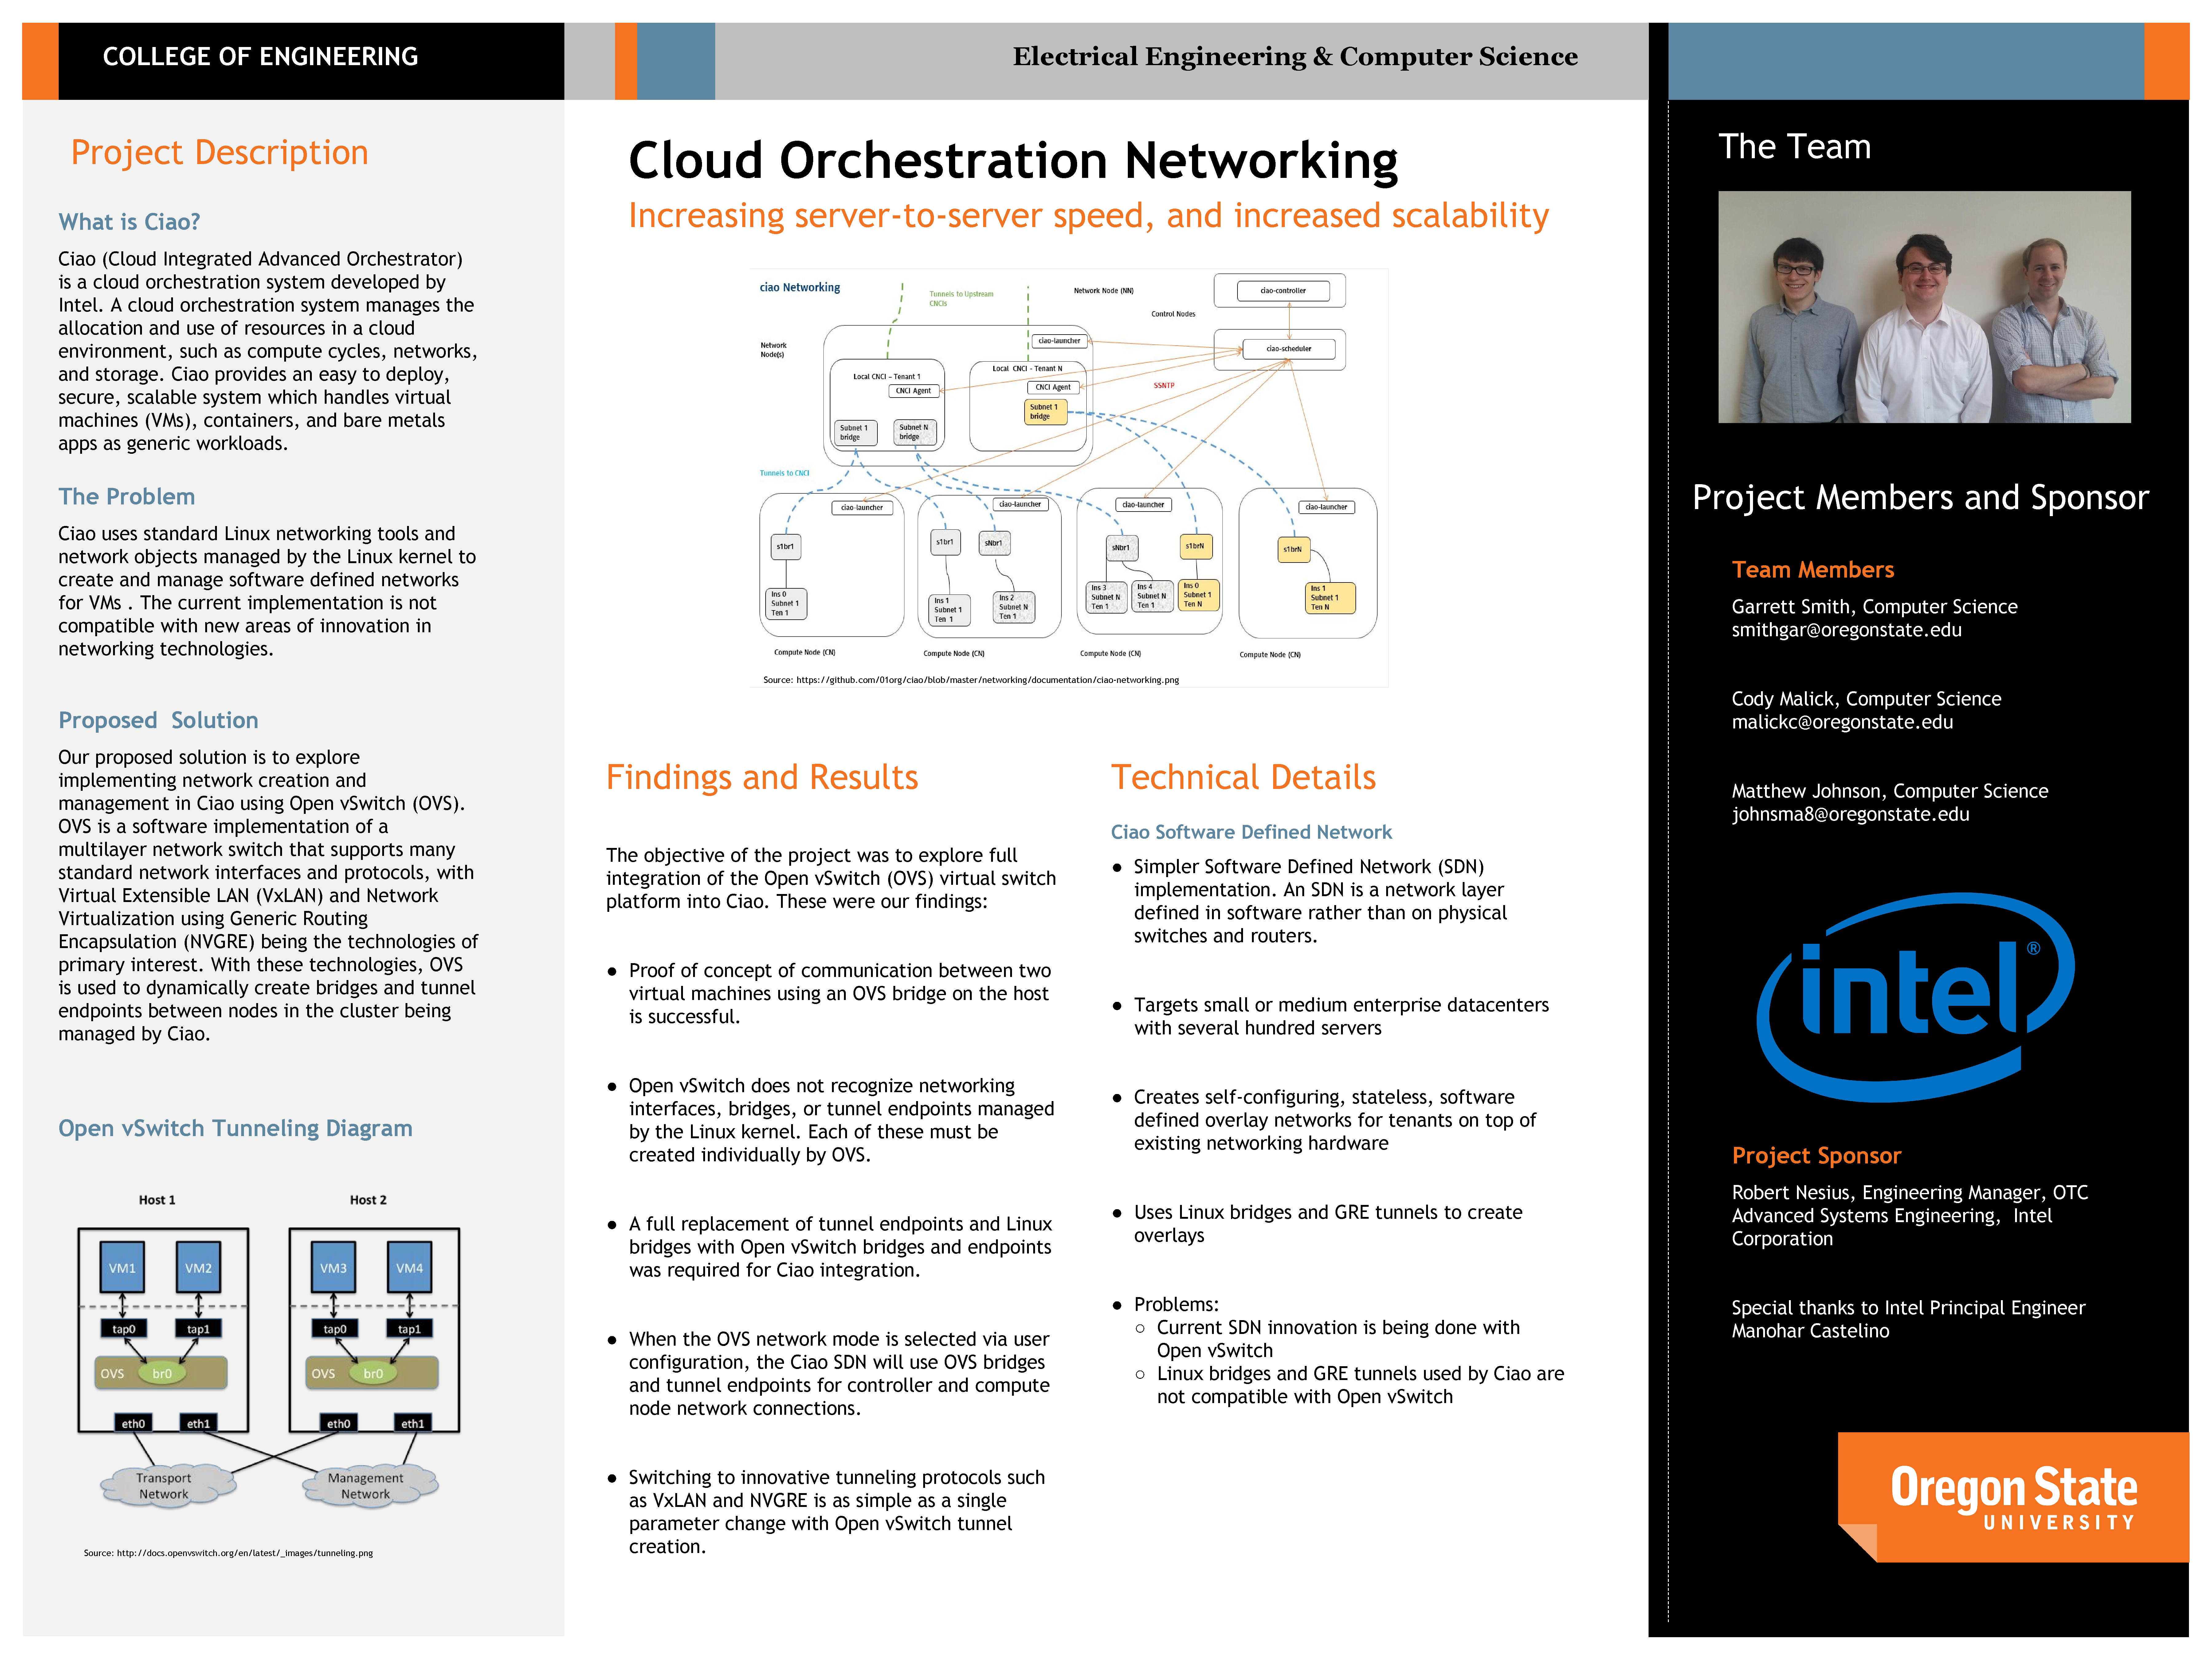
\includepdf[landscape=true]{docs/poster.pdf}

\section{Project Documentation}
\subsection{Project Overview}
Ciao is a cloud orchestrator, and requires a basic setup of five machines: a deployment node, a control node running Ciao, a network node, and two compute nodes. Because developing software on a cluster can be difficult, we use Ciao-Down, a CLI utility for single machine development.
\subsection{Installation Instructions}
% We should give instructions on Ciao-down
The simplest way to run Ciao is in single VM mode with ciao-down.
We had issues running Ciao in a multiple machine environment due to DHCP issues, but you are welcome to give it a try.
The main issue we were seeing was caused by the OSU network. Ciao uses the external DCHP server to assign IP addresses
to the instances it spins up. These instances have generated MAC addresses. The OSU network will only lease an IP
address if the MAC address is registered with the university IT department. Our problem was that since the generated
MAC addresses were not registered with the university the instances were never assigned IP addresses and were therefore
inaccessible. If you want to run Ciao in a cluster Intel provides very detailed instructions.
Manual deployment instructions can be found at \url{https://clearlinux.org/documentation/ciao/cluster-setup.html}.
Instructions for deployment via an Ansible playbook can be found at\\
\url{https://clearlinux.org/documentation/ciao/deployment/deployment.html}.

\subsection{Running Ciao-Down}
\begin{itemize}
    \item Download the master version of Ciao by running 
          \texttt{go get github.com/01org/ciao}
    \item Change directories into the Ciao git repo
    \item Add our Ciao repo as a remote with \texttt{git remote set-url origin git@github.com:matthewrsj/ciao.git}
    \item \texttt{Run git fetch} to get our changes
    \item Checkout the ovsdev branch with \texttt{git checkout ovsdev}
    \item Build ciao-down with \texttt{go get github.com/01org/ciao/testutil/ciao-down}
    and \texttt{\$GOPATH/bin/ciao-down prepare}
    \item Connect to the ciao-down VM with \texttt{\$GOPATH/bin/ciao-down connect}
    \item When you connect to the VM it will provide you with instructions to finish setting up your
          environment and run a workload.
    \item To power off the VM run \texttt{ciao-down stop}
    \item To remove the VM run \texttt{ciao-down destroy}
\end{itemize}


\subsection{Project Software Requirements}
\begin{itemize}
    \item CPU that supports nested KVM. You must have nested KVM enabled as well.
    \item Ubuntu 16+, Arch Linux, Fedora. Other distributions may work but are not tested.
    \item Golang 1.8 or newer.
    \item Ciao-down requires several other binaries. If you are missing any ciao-down will prompt you to install them.
\end{itemize}
\subsection{Additional References}
% Link to ciao repo, official documentation, and anything else we want to include

% Group section
\section{"How did you learn new technology"}
Due to the nature of the project, one of the best ways to learn was to dive in. While we were very hands on, the Ciao documentation was critical to learning and understanding the code base. 

Open vSwitch was another challenging technology to pick up. Software defined networking is a highly technical subject. There were not a lot of specific websites that provide thorough examples and documentation on the technology. We did gain insight into OVS by reading the original IEEE RFC 7047 for the management database\cite{rfc7047}.

The official Golang documentation was another critical source of information for us. Without it, we wouldn't have been able to write the code that we did. It's available online at \url{https://golang.org/ref/spec}.

Last, but certainly not least, Manohar Castelino was a huge source of domain knowledge in relation to Ciao. A principle engineer and primary author of Ciao networking, Manohar was extremely helpful in helping us over difficult hurdles this year.

% How did you learn new technology?
% What web sites were helpful? (Listed in order of helpfulness.)
% What, if any, reference books really helped?
% Were there any people on campus that were really helpful?

\section{"What did you learn?"}
% Individual Assignment

%Questions to answer:
%What technical information did you learn?
%What non-technical information did you learn?
%What have you learned about project work?
%What have you learned about project management?
%What have you learned about working in teams?
%If you could do it all over, what would you do differently?

\subsection{Matthew}

%What technical information did you learn?

At the beginning of the project I had a vary basic understanding of software defined networking, cloud orchestration
or networking in general. Although I understood the concepts, I had no experience with the actual implementation
details of any of the technologies we worked with.

In a general sense, I learned a lot about how software defined networking actually works in practice and specifically
how Ciao's implementation works. Cloud orchestration is a complicated problem that Ciao is approaching in an innovative
way.

To be more specific, I obviously learned a ton about Open vSwitch and other new and innovative SDN technologies such
as VXLAN and NVGRE tunneling protocols. I also learned a lot about the Go programming language and learned to appreciate
its error handling and overall philosophy. Some technical experience I gained that was indirectly related to our project
was a better understanding of the various Linux networking tools available that we used to debug the issues we saw during 
project.

%What non-technical information did you learn?

I also gained some non-technical skills during my work on this project. I learned to be more accepting of scope changes
due to the major scope change we had during Winter Term. I also learned to never trust my assumptions about how something
should work, because most likely those assumptions will be wrong. Connecting the two, I learned that incorrect assumptions
can lead to major scope changes in your project if not careful.

%What have you learned about project work?

About project work, I've learned that not everyone has the same understanding of the technical aspects of the project.
For example, I had a much lower understanding of advanced networking than Garrett and a less complete grasp of the Go
programming language. On the other hand, because I read through the Ciao code more closely I understand the inner-workings
of Ciao better than either of them. When working on a project together this information must be freely shared in order
to achieve a successful collaboration.

%What have you learned about project management?

Project management and leadership is another area where everyone in the group gained
experience. We all worked well together and different members took responsibility for
different aspects of the project. We learned to rely on each other to stay on task and
focused.

%What have you learned about working in teams?

One thing that really helped us keep our work progressing was agreeing on a specific time
to meet every week. Everyone on the team took it very seriously and showed up to all the
team meetings. This kept everyone accountable for work being done and kept us motivated
every week.

%If you could do it all over, what would you do differently?

If I could do the project all over again, I would mistrust assumptions from the start of the project. This would have
saved us several weeks of work before the scope change. Additionally, we tried to not bother our clients with technical
questions too much since this was our project to complete. I did not want it to seem like we were relying on our very
technical clients (one of them a Principal Engineer at Intel) to do our work for us. In hindsight it might have been
better to ask those technical questions so they could at least point us in the right direction. While we did ask
several technical questions throughout the year, asking more might have saved us some troubleshooting time.

\subsection{Garrett}

%What technical information did you learn?
This project was very technical and as a result I received experience with a variety of tools, technologies, and technical concepts.
Software define networking was the main technical point of the project, but along the way 
we worked with Go, Open vSwitch, general Linux networking utilities, network tunneling protocols, virtual machines, docker, and Ciao.
The hands on experience I received with these tools and technologies is amazing.

To start with, setting up Ciao was great for learning how clouds are created and managed.
To deploy Ciao to a cloud you as the user only have to install the Ciao software on one machine in your cloud. Ciao will take care of finding the other machines you want it deployed to, and installing its self. 
You set up your servers with a user and a key that can be used to SSH into the server
, and give Ciao the user names and keys via configuration.
It takes care of installing all of the components it needs to manage the machines.
This makes a ton of sense looking back on it, but
my initial thought was that you would need to set up a client on each machine in the cloud, and have it report back to the Ciao control node you are using to manage the cloud.
This is a clever system, and one that makes a lot of sense once I saw how it works, but not one that was initially intuitive to me.


Prior to this project I had used Go for a couple of toy personal projects, but nothing serious.
Working on Ciao gave me actual experience with Go in a large scale project. I learned how large Go projects are structures, and how the different packages are set up.
The project also gave me practice code in Go which is the best way to get comfortable with a language.

Before we could replace the Linux bridges, and Linux created GRE tunnels that Ciao was using we had to understand what it was doing. This meant learning how Linux bridges work, and how to create GRE tunnels with the basic Linux utilities. Once we figured this out we where able determine what the networking sections of Ciao were doing, and where we needed to make our changes. That process taught me a lot about using Linux networking utilities such as \texttt{ip}.

Another important piece of technology I learned about was Open vSwitch. We had to know how to use it to integrate it into Ciao. I spent a few days running through some demos, and figuring out how to set up bridges and tunnels with Open vSwitch. I feel comfortable using it now, and I would consider using it in other projects if I needed a software switch.

%What non-technical information did you learn?
On the non technical front I improved my communications skills because I had to be in regular contact with my team to keep them up to date on what I was working on, any issues I ran into, and my progress.

%What have you learned about project work?
Project work is very different from school work. I learned just how much planning goes into a project before any work can start, and how structured it is. Working on the Capstone project involved a very constant stream of work which is different from traditional school projects which are short bursts of work. Overall I enjoyed working on the project. It was long enough lived that I felt invested int it, and I'm proud of my accomplishments which is not something I get very much from school work.

%What have you learned about project management?
This was not my first time working on a team or on a large project, but it was my first time working on a project of this scale where I was one of the people in charge.
There is a lot of planning involved, and you have to be flexible when something unexpected occurs.
We had a large scope change and it threw our initial plan off track.
Working around issues as they come up, and updating your plan if you need to is really important when managing a project.

%What have you learned about working in teams?
Having a good team can make or break a project. 
We had a hard project, but we had an amazing team. 
Cody and Matthew were great to work with on a number of levels.
We all stayed in frequent communication via group text chat, and met up regularly.
This made it easy to keep up with who was working on what, and their progress.
A structured schedule and regular communication make working in a group a lot easier.

%If you could do it all over, what would you do differently?
If I were doing this all over again I would take more time to prototype and figure out exactly what technical questions we need to answer, and what issues we need to resolve before diving in. We had a scope change because we had to do a full replacement of the Linux bridges in Ciao with Open vSwitch instances which was a surprise part way through Winter term. I would try to prepare for that. In a more generalized sense I would try to figure out what assumptions we were making and figure out if they are correct as soon as possible.


\subsection{Cody}
%Questions to answer:
%What technical information did you learn?
This project encompassed a few major areas that I had no previous experience with. From a technical perspective, cloud orchestration and software defined networking were two big knowledge gaps for me. Also, as a side effect of learning SDN, I learned quite a bit about networking in general. While being familiar with the Go programming language, commonly referred to as Golang, I improved as a Go developer significantly this year. 

``Cloud orchestration'' is a bit of a buzzword. Going into the project, I had had no prior experience in the area. Jumping from no knowledge to working on the code base of a cloud orchestrator was quite a bit of fun. While we didn't have to touch the algorithm that operated Ciao, we had to understand the fundamentally structure of the software we were altering. I picked up quite a bit of information reading through the Ciao docs, and through reading articles about basic goals of Ciao.

Learning software defined networking, as a topic, was pivotal to implementing the project. Ciao uses software defined networking to track the state of the network internally. With this capability, it can spin up VMs or containers at will, and allow the user to not worry about which server they run on. Understanding how SDN's abstract the physical layer was interesting and fulfilling to learn. As a side effect of having to learn SDN, my general understanding of networking improved substantially.

Go has quickly become one of my favorite languages. It enforces simplicity and performance, while providing fantastic multi-threading and concurrency constructs. As our resident Golang expert, I had to convey knowledge to Garrett and Matthew as we moved through development. The best way of learning something is by explaining it to others!

%What non-technical information did you learn?
From a non-technical standpoint, my ability to plan and design projects in general have improved over the year. While many did not enjoy the documentation portion of the project, I felt I grew significantly as, not only an engineer, but an architect. 

Another area I felt greatly improved was public speaking. While there was a limited amount of it this year, standing up and explaining our project to people of different backgrounds and cultures was fun and challenging. Through explanation of the project to others, I gained a better understanding of our own project and how it fit into the bigger picture.

%What have you learned about project work?
Working on projects is not a new experience to me, but I learned quite a bit about design this year. Rather than just jumping in, figuring out exactly what we wanted to do helped us in the long run. While we had a large scope change, we were able to use most of our original design to execute the project. Each member of our team took individual planning and execution rolls. One of the big keys to our success this year is that we planned out our weekly meeting times. More importantly, we stuck to those times. Every member of the group showed up and executed. While I feel that we spent more time planning than we needed to, it paid off significantly at the end of the year. We were much more relaxed when we knew exactly what was going to happen.

%What have you learned about working in teams?
From a group work perspective, I found out what it meant to be part of a team that has synergy. In the past, I've worked with teams that worked well together, and others that did not. Matthew and Garrett were a pleasure to work with, and I have greatly enjoyed dividing class work, and tackling problems together. Overall, I think that the people you work with is far more important that the subject you're working on.

%If you could do it all over, what would you do differently?
Overall, I feel we did extremely well. If I were to do it over again, I would spend more time getting familiar with our code base in fall. Quite a few of our original roadblocks resulted from unfamiliarity with how Ciao is developed, and what tools were used in that development process.

\section{Conclusion}
This year has been challenging, but a large growing experience for our team. Working on Ciao has given each of our team a chance to learn, from new technologies to design work. We would like to thank Kevin, Kirsten, and Intel for their support this year. We are satisfied with the work we've done this year, and are looking forward to our commencing our work in software engineering.

\bibliographystyle{IEEEtran}
\bibliography{prog}

\section{Appendix A}
% Essential Code Listings
The following listings illustrate bridge creation with OVS. A similar method is used for tunnel endpoint creation.

\begin{lstlisting}[caption=Calling the OVS command tool]
func vsctlCmd(args []string) error {
	_, err := exec.Command("ovs-vsctl", args...).Output()

	if err != nil {
		glog.Error("vsctlCmd failed: " + err.Error())
		return err
	}

	return nil
}
\end{lstlisting}

\begin{lstlisting}[caption=Creating an OVS bridge]
func createOvsBridge(bridgeId string) error {
	// Example: ovs-vsctl add-br ovs-br1
	args := []string{"add-br", bridgeId, "--", "set", "bridge", bridgeId, "datapath_type=netdev"}

	// Execute command
	if err := vsctlCmd(args); err != nil {
		return err
	}

	return nil
}
\end{lstlisting}

\begin{lstlisting}[caption=Destroying an OVS bridge]
func destroyOvsBridge(bridgeId string) error {
	// Example: ovs-vsctl del-br ovs-br1
	args := []string{"del-br", bridgeId}

	if err := vsctlCmd(args); err != nil {
		return err
	}

	return nil
}
\end{lstlisting}

The following code listing is an example of how network mode switching was handled in Ciao.

\begin{lstlisting}[caption=Network mode switching]
switch b.Mode {
case GreTunnel:
	bridge := &netlink.Bridge{LinkAttrs: netlink.LinkAttrs{Name: b.LinkName}}
	if err := netlink.LinkAdd(bridge); err != nil {
		return netError(b, "create link add %v %v", b.GlobalID, err)
	}
	
	link, err := netlink.LinkByName(b.LinkName)
	if err != nil {
		return netError(b, "create LinkByName %v %v", b.GlobalID, err)
	}
	
	brl, ok := link.(*netlink.Bridge)
	if !ok {
		return netError(b, "create incorrect interface type %v %v", b.GlobalID, link)
	}
	
	b.Link = brl
	if err := b.setAlias(b.GlobalID); err != nil {
		err1 := b.Destroy()
		return netError(b, "create set alias [%v] [%v]", err, err1)
	}
	
	return nil
case OvsGreTunnel:
	if err := createOvsBridge(b.GlobalID); err != nil {
		return err
	}
	
	return nil
default:
	return netError(b, "Create Bridge: unknown network mode %v, bridge %v", b.Mode, b.GlobalID)
}

\end{lstlisting}

This final listing shows the data structure used to store information on the bridge object.

\begin{lstlisting}[caption=Ciao bridge object and supplementary OvsBridge object]
// Bridge represents a ciao Bridge
type Bridge struct {
	Attrs
	Link *netlink.Bridge
}

// OvsBridge represents a ciao bridge created via ovs-vsctl
type OvsBridge struct {
	Attrs
}
\end{lstlisting}


\section{Appendix B}
% Anything Else
\begin{figure}[H]
\caption{The Golang Gopher}
\makebox[\textwidth][c]{
\includegraphics[scale=2]{gopher}}
\end{figure}

\end{document}
